% Šablona pro maturitní práci Gymnázia Jírovcova 8, České Budějovice
% Autoři šablony: Jonáš Havelka, Michal Kočer, Daniel Sýkora
% Typ dokumentu: report
% veškeré úpravy v soubor MP.sty (styl maturitní práce)
\documentclass[12pt]{report}
% %%%%%%%%%%%%%%%%%%%%%%%%%%%%%%%%%%%%%%%%%%%%%%%%%%%%%%%
\usepackage{listingsutf8}
\usepackage{float}
\usepackage{graphicx}
\usepackage{subcaption}
\usepackage{MP}
\setlength{\parindent}{15pt} % Nastaví odsazení prvního řádku odstavce na 15pt
						  % Import stylu maturitní práce
\author{Kryštof Maxera}                  % AUTOR PRÁCE
\title{Konstrukce dronu}    % NÁZEV PRÁCE
\date{14. února 2025}                 % DATUM ODEVZDÁNÍ PRÁCE
\vedouci{Dr.rer.nat Michal Kočer} % VEDOUCÍ PRÁCE
\place{V Českých Budějovicích}
\skolnirok{2024/2025}                  % ŠKOLNí ROK
\logo{
\includegraphics[scale=1.25]{GJ8_logotyp}} %Logo školy
%%%%%%%%%%%%%%%%%%%%%%%%%%%%%%%%%%%%%%%%%%%%%%%%%%%%%%%%%%%%%%%%%%%
\begin{document} %%%%%%% začátek dokumentu
%%%%%%%%%%%%%%%%%%%%%%%%%%%%  Titulní stránka + úvodní povinné stránky
\pagenumbering{roman}                   % číslování stránek římskými číslicemi
	\mytitlepage						% Vygenerování titulní strany
	
	\prohlaseni{
		Prohlašuji, že jsem tuto práci vypracoval samostatně s vyznačením všech použitých pramenů.
	}	
	
	\abstrakt{
		V této práci se zabýváme problematikou konstrukce kvadrokoptéry ve spojení s mikrořadičem Arduino. Rozebíráme jak fungují její základní komponenty a principy fyziky letu. Praktická část práce se zaměřuje na návrh a sestavení skutečné kvadrokoptéry. 
	}{
		Kvadrokoptéra, konstrukce dronu, fyzika letu dronu, Arduino 
	}
	
	\podekovani{
		\lipsum[2]						% Poděkování
	}
	
   {\tableofcontents\newpage}			% Obsah
	
%%%%%%%%%%%%%%%%%%%%%%%%%%%% VLASTNÍ PRÁCE
\addtocounter{page}{1}		% Posunutí countru stránek
\pagenumbering{arabic}		% Číslování stránek arabskými číslicemi
\chapter*{Úvod}     % úvod práce 
	
\lipsum[1]	
	
%%%%%%%%%%%%%% TEORETICKÁ ČÁST %%%%%%%%%%%%%%%%%%	
\part[Úvod do světa dronů]{Úvod do světa dronů}  % název teoretické části (nenechávejte Teoretická část)

\chapter[Definice a charakteristika dronů]{Definice a charakteristika dronů}

Dron je definován jako zařízení nebo stroj schopný vykonávat úkoly bez nutnosti přímé fyzické přítomnosti člověka. Tato zařízení lze rozdělit do dvou základních kategorií.\\
První kategorii tvoří plně autonomní roboti, u jichž je přítomnost člověka vyžadována primárně z kontrolních a bezpečnostních důvodu. Pilot nebo operátor zde většinou nezasahuje do aktivního řízení, ale v případě potřeby může převzít kontrolu. Typickým příkladem jsou autonomní bezpilotní letadla s možností vzdáleného ovládání nebo samořízené motorové vozidlo, které ke svému provozu nepotřebuje řidiče přítomného ve vozidle.\\
Druhá kategorie je pro veřejnost známější. Zařízení v této kategorii se také nazývají drony, přestože se jedná dálkově ovládaná zařízení, která nejsou plně autonomní. Do této skupiny patří široce známé kvadrokoptéry a další multikoptéry, stejně jako autíčka na dálkové ovládání.\\
Důvodem časté záměny těchto dvou kategorií je překrývání některých funkcí, neboť i dálkově ovládané kvadrokoptéry využívají automatické systémy, například pro samovyvažování, které jsou nezbytné pro jejich stabilní let.\cite{mainbook}\\

Drony lze obecně rozdělit do několika hlavních skupin na základě prostředí, ve kterém operují:
\begin{itemize}
	\item \textbf{Bezpilotní letadla} (UAVs - Unmanned Aerial Vehicles)
	\item \textbf{Bezpilotní pozemní vozidla} (UGV - Unmanned Ground Vehicle)
	\item \textbf{Hladinová plavidla bez posádky} (USV - Unmanned Surface Vehicle)
	\item \textbf{Dálkově ovládaná podvodní vozidla} (ROUV - Remotely Operated Underwater Vehicles)
	\item \textbf{Bezpilotní kosmické lodě} (Uncrewed spacecraft)
\end{itemize}

Přestože označení dron lze použít pro širokou škálu zařízeních, pro širokou veřejnost je toto slovo primárně spjaté s dálkově ovládanými bezpilotními letadly. Samo o sobě však toto označení není chybné. V této práci se zaměřujeme na konstrukci kvadrokoptéry, která spadá do kategorie bezpilotních letadel. O té práce pojednává podrobněji. \cite{mainbook}

\section[Bezpilotní letadla]{Bezpilotní letadla}
Bezpilotní letadlo (UAV) je definováno jako zařízení určené k provozu ve vzdušném prostředí, které je buď řízeno dálkově operátorem, nebo schopno autonomního letu díky integrovanému softwaru a palubním senzorům.\\
Tato zařízení využívají pokročilé technologie pro navigaci, stabilizaci, komunikaci a sběr dat, přičemž jejich provozní komponenty se liší v závislosti na specifickém účelu použití. Obecně však tato zařízení obsahují senzory nezbytné pro stabilizaci letu, jako je gyroskop a akcelerometr, spolu se senzory či moduly umožňujícími komunikaci. Komunikační technologie obvykle zahrnují přenos dat prostřednictvím rádiových vln, Wi-Fi, nebo mobilních sítí.\\
Tato zařízení lze dále klasifikovat na základě specifických parametrů, jako je typ konstrukce křídla, hmotnost, zdroj napájení či funkční zaměření.\\

\begin{figure}[H]
	\centering
	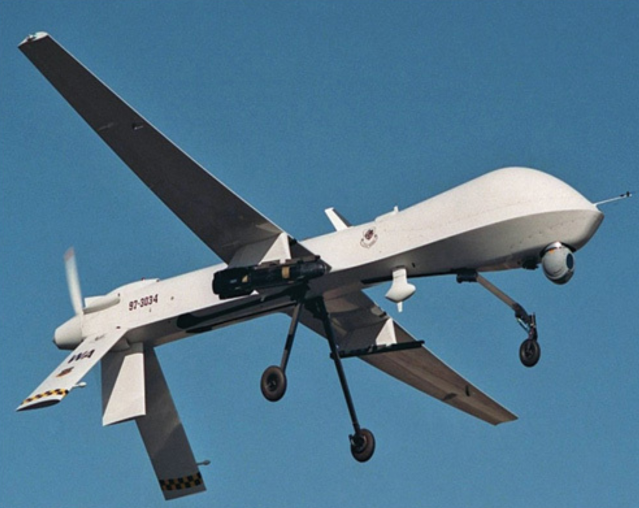
\includegraphics[width=0.5\linewidth]{uav.png}
	\caption{Bezpilotní letadlo General Atomics MQ-1 Predator \cite{mainbook}}
	\label{fig:uav.png}
  \end{figure}

Při klasifikaci na základě typu konstrukce křídla lze bezpilotní letadla rozdělit do dvou hlavních skupin:
\begin{itemize}
	\item Rotorová letadla - zahrnující jednorotorové a vícerotorové varianty, jako jsou trikoptéry, kvadrokoptéry, hexakoptéry a oktokoptéry.
	\item Letadla s pevnými křídly - zahrnují drony, které vyžadují pohyb vpřed k generování vztlaku pomocí křídel. Patří sem také hybridní drony s vertikálním vzletem a přistáním, jež nevyžadují přistávací dráhu.
\end{itemize}

Zařazení na základě zdroje napájení:
\begin{itemize}
	\item Bateriový pohon - nejčastěji lithium-polymerové (Li-Po) nebo lithium-iontové (Li-Ion) baterie
	\item Benzínový pohon - spalovací motor poháněný benzínem
	\item Vodíkový pohon - napájení je zajištěno vodíkovými palivovými články, které generují elektrickou energii chemickou reakcí
	\item Solární pohon - solární panely umístěné na povrchu dronu zajišťují nepřetržité nabíjení během letu
\end{itemize}

Zařazení na základě způsobu použití:
\begin{itemize}
	\item rekreační využití
	\item letecká fotografie a videografie
	\item pátrací a záchranné operace
	\item vojenský průmysl
	\item stavební průmysl, monitorování a měření
	\item zemědělství
	\item dopravní a logistické služby
\end{itemize}

Tato skupina zařízení byla po dlouhou dobu spojována především s vojenským průmyslem. V současnosti však díky široké škále aplikací nacházejí stále větší uplatnění i v civilních oblastech jako je průmysl, zemědělství nebo vědecký výzkum. Díky klesajícím cenám se osobní kvadrokoptéry stávají stále populárnějšími také pro rekreační účely. \cite{mainbook} \cite{whatisadrone}\\

\section[Bezpilotní pozemní vozidla]{Bezpilotní pozemní vozidla}
Jedná se o pozemní vozidla bez potřebné fyzické přítomnosti člověka. Ve srovnání se vzdušnými bezpilotními drony jsou mnohem jednodušší na konstrukci. Tato vlastnost přispívá k jejich širokému využití napříč různými sektory. Lze je nalézt například v zemědělství jako samosklízecí traktory, v oblasti samořídicích dopravních prostředků, v těžebním průmyslu, v automatizovaných skladech s roboty pro transport zboží nebo v úklidovém sektoru, kde se využívají jako autonomní vysavače. Své uplatnění nacházejí také ve vojenském sektoru. \cite{mainbook}

\section[Hladinová plavidla bez posádky]{Hladinová plavidla bez posádky}
Plavidla pohybující se po mořské nebo sladkovodní hladině. Často jsou využívána pro těžební operace na moři, vědecký výzkum či monitorování vodních ekosystémů. Významné je také jejich vojenské využití. Tato zařízení používají pro komunikaci obdobné technologie jako bezpilotní letadla. \cite{mainbook}

\section[Dálkově ovládaná podvodní vozidla]{Dálkově ovládaná podvodní vozidla}
Podvodní zařízení určená převážně pro průzkumné a vědecké účely. Představují klíčový nástroj pro studium mořského prostředí. Jejich fungování se však výrazně liší od ostatních autonomních systémů, a to kvůli technickým výzvám spojených s provozem ve velkých hloubkách. V těchto podmínkách je použití rádiových vln pro komunikaci téměř nemožné kvůli jejich omezené prostupnosti vodou. Namísto bezdrátové komunikace jsou proto tato zařízení spojena s mateřskou lodí nebo ponorkou pomocí robustního kabelu, který slouží nejen jako přenosové médium pro data a jako zdroj energie. \cite{mainbook}

\section[Bezpilotní kosmické lodě]{Bezpilotní kosmické lodě}
Vesmír představuje ideální prostředí pro využití dronů. Jedná se o místo, které je význačné svou nehostinnostní pro lidskou přítomnost. Vesmírné drony nabízejí méně rizikové řešení pro dosažení různých cílů bez nutnosti návratu zařízení zpět na Zemi. Místa, kde se využívají, zahrnují kosmický prostor, kde slouží k prozkoumávání vzdálených objektů, povrchy nehostinných planet, kde fungují jako rovery, a oběžnou dráhu Země, kde podporují fungování klíčových technologií, jako je například GPS. \cite{mainbook}\\

Využití všech těchto typů dronů má společnou vlastnost. Jejich využití je na místech, kde lze drahou pracovní sílu člověka nahradit automatickým zařízením nebo místech, které jsou příliš riskantní pro přítomnost člověka. Jejich nasazení se neustále rozšiřuje a lze předpokládat, že v budoucnu bude jejich význam dále narůstat.

\chapter[Anatomie multikoptéry]{Anatomie multikoptéry}
Každá multikoptéra, ať už profesionálně vyrobená nebo sestavená v domácích podmínkách, se liší svým konstrukčním hardwarem. Většinu těchto zařízení však spojuje použití podobných klíčových komponent. Tato kapitola se zaměřuje na podrobný popis nejběžnějších součástek, které zároveň byly využity při konstrukci v praktické části práce.

\section[Rám]{Rám}
Rám dronu tvoří základní konstrukční prvek, který drží všechny komponenty pohromadě. Typ rámu použitý u dronu má zásadní vliv na jeho celkové vlastnosti. Klíčovým aspektem při výběru a návrhu rámu je nalezení optimálního poměru mezi hmotností, velikostí a pevností. Je důležité, aby konstrukce byla co nejvíce odolná vůči nárazům a pádům, zároveň však nezvyšovala zbytečně hmotnost zařízení. Tento vyvážený design hraje významnou roli ve stabilitě, ovladatelnosti a životnosti dronu.

\begin{figure}[H]
	\centering
	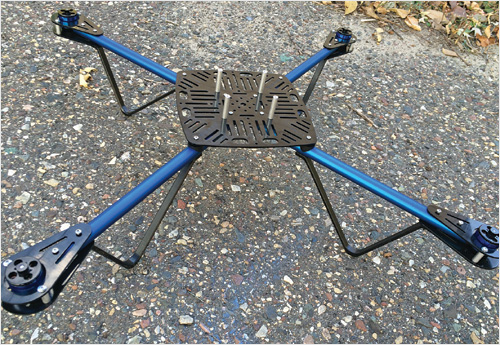
\includegraphics[width=0.65\linewidth]{ram.jpg}
	\caption{Rám vyrobený z plastu a hliníku \cite{mainbook}}
	\label{fig:ram.jpg}
  \end{figure}

\subsection[Tvar]{Tvar}
První klíčovou vlastností rámu je tvar. Konstrukce rámu musí odpovídat počtu vrtulí, což vyžaduje adekvátní počet ramen. Například trikoptéry disponují třemi rameny, hexakoptéry šesti, zatímco nejběžnější kvadrokoptéry mají čtyři ramena. Důležitým konstrukčním aspektem je také úhel mezi jednotlivými rameny, který ovlivňuje nejen stabilitu a letové vlastnosti dronu, ale také případné zorné pole připevněné kamery.

\subsection[Materiál]{Materiál}
Výběr materiálu rámu výrazně ovlivňuje dvě klíčové vlastnosti dronu: hmotnost a odolnost. Existuje široká škála materiálů vhodných pro konstrukci rámu.\\

Nejčastěji používané materiály zahrnují:
\begin{itemize}
	\item Uhlíkové vlákno - vynikající pevnost a nízká hmotnost, vysoká cena, pro profesionální konstrukce
	\item Dřevo - snadná dostupnost, výborná tvarovatelnost, vhodné pro malé multikoptéry
	\item Hliník - vysoká pevnost a odolnost, nízká cena, vysoká hmotnost
	\item Pěna - převážně u malých dronů díky své nízké hmotnosti, omezená stabilita
	\item Plast - levný, lehký a snadno tvarovatelný materiál, možné použití 3D tisku
\end{itemize}

\subsection[Velikost]{Velikost}
V neposlední řadě je potřeba zvolit správnou velikost dronu. Obecně platí, že s rostoucí velikostí se zvyšuje jak jeho hmotnost, tak zároveň i jeho stabilita. Volba optimální velikosti závisí na požadovaných letových vlastnostech a plánovaném zatížení dronu. \cite{mainbook} \cite{dojo} \cite{ultimateguide}

\section[Motory]{Motory}
Motor se skládá ze dvou částí, rotoru a statoru. Rotor je ta část motoru, která se při běhu točí a stator je ta část, která stojí na místě.

\subsection[Inrunner a outrunner]{Inrunner a outrunner}
Motory lze rozdělit do dvou podkategorií: inrunner a outrunner, přičemž klíčový rozdíl spočívá v umístění rotoru a statoru.\\
\textbf{Inrunner motory} mají rotor uvnitř statoru, otáčí se pouze hřídel motoru a vnější plášť zůstává statický. Tyto motory se vyznačují vysokými otáčkami (vyšší kV) a nízkým točivým momentem, což je ideální pro situace vyžadující rychlost.\\
\textbf{Outrunner motory} mají rotor na vnější straně statoru, takže se otáčí celý plášť motoru. Tento design poskytuje nižší otáčky (nižší kV), ale vyšší točivý moment, což je ideální pro pohon vrtulí dronů nebo elektrokol. 

\begin{figure}[H]
	\centering
	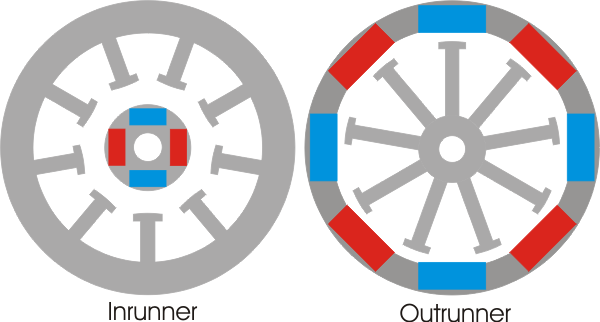
\includegraphics[width=0.6\linewidth]{inrunner-outrunner.png}
	\caption{Rozdíl mezi inrunner a outrunner motorem \cite{rozum}}
	\label{fig:inrunner-outrunner.png}
  \end{figure}

\subsection[Kartáčové a bezkartáčové motory]{Kartáčové a bezkartáčové motory}
Jedná se o dva hlavní druhy motorů, lišící se způsobem přenosu energie a účinností.\\
\textbf{Kartáčové motory} (brushed motors) používají mechanické kartáče k přenosu elektrické energie na rotor, kde jsou umístěny cívky. Stator je tvořen permanentními magnety. Proud procházející cívkami rotoru vytvoří magnetické pole odpuzované magnety na statoru tak, že motor generuje točivý moment. Tento design je jednoduchý a levný, ale méně účinný kvůli tření kartáčů, což způsobuje vyšší opotřebení a ztráty energie.\\
\textbf{Bezkartáčové motory} (brushless motors) mají cívky na statoru a rotor tvořený permanentními magnety. Energie je přenášena elektronicky pomocí regulátorů otáček (ESC), které ve správný čas mění polaritu cívek tak, aby odpuzovaly permanentní magnety na rotoru. Tento způsob eliminuje tření kartáčů. Bezkartáčové motory jsou účinnější, spolehlivější a vhodné pro aplikace vyžadující vysoký výkon a přesnost. Často se využívají například u dronů nebo elektromobilů.


\begin{figure}[H]
	\centering
	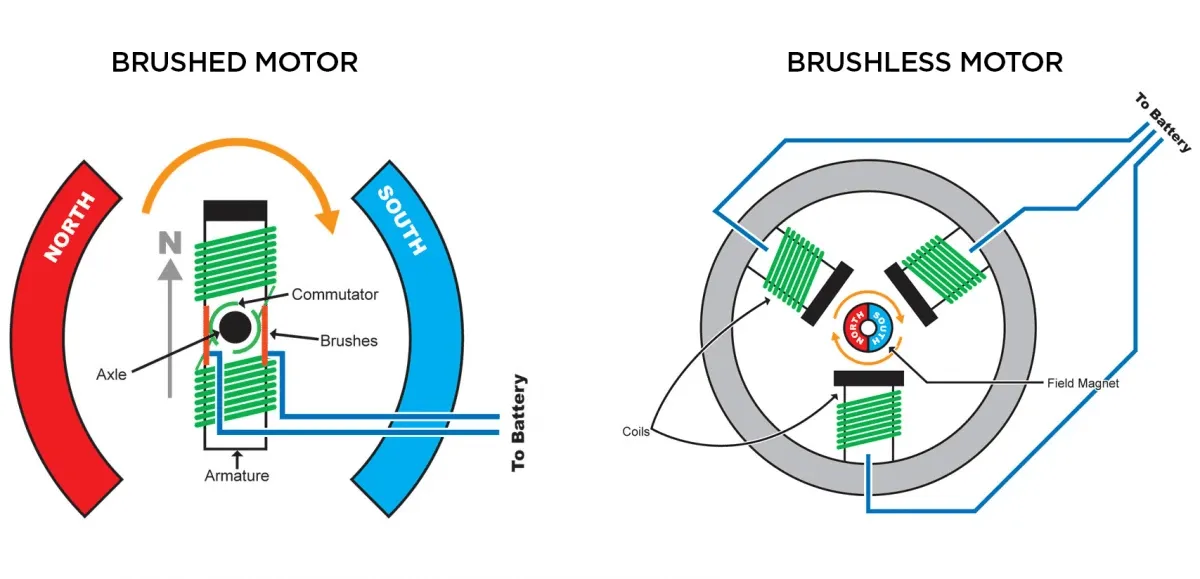
\includegraphics[width=0.9\linewidth]{brushed-brushless.png}
	\caption{Rozdíl mezi kartáčovým a bezkartáčovým motorem \cite{rozum}}
	\label{fig:brushed-brushless.png}
  \end{figure}

\subsection[AC a DC]{AC a DC}
Klíčové je také správné spárování baterie s motorem. Baterie obvykle využívají stejnosměrný proud (DC), zatímco bezkartáčové motory střídavý proud (AC). V takových případech je nezbytné zvolit vhodný regulátor otáček (ESC), který zajistí správnou transformaci a distribuci elektrického proudu motorům. Kartáčové motory ke svojí funkci vyžadují stejnosměrný proud. \cite{mainbook} \cite{dojo} \cite{ultimateguide} \cite{motors}

\section[Vrtule]{Vrtule}

Vrtule fungují podobně jako šroub. Jejich lopatky se při otáčení “zavrtávají” do vzduchu a vytvářejí tak sílu, která pohání objekt vpřed.\\
Používají se primárně dvě varianty vrtulí, které se liší směrem otáčení. První varianta se otáčí po směru hodinových ručiček (CW), zatímco druhá proti směru hodinových ručiček (CCW). Kombinace obou varian vrtulí napomáhá k vyvážení a stabilizaci zařízení. \cite{mainbook} \cite{dojo}

\section[Řídicí jednotka]{Řídicí jednotka}

Řídicí jednotku (flight controller) lze přirovnat k „mozku“ celého dronu. Její hlavní funkcí je ovládání a automatické vyvažování dronu. Zajišťuje, aby dron zůstal stabilní i v obtížných podmínkách, jako je vítr nebo nerovnoměrné rozložení hmotnosti. Díky tomu se pilot nemusí soustředit na neustálé drobné korekce, což usnadňuje manévrování.\\

Nejběžnější senzory součástí řídicí jednotky:
\begin{itemize}
	\item Akcelerometr -  Měří zrychlení ve třech osách (x, y, z) a pomáhá určit směr gravitace, což je nezbytné pro vyhodnocení naklonění dronu.
	\item Gyroskop - Sleduje rotaci a úhlové změny dronu, což umožňuje rychlé a přesné úpravy pro udržení stability.
\end{itemize}

Řídicí jednotka přijímá data ze senzorů a na jejich základě upravuje výkon jednotlivých motorů. \cite{mainbook}

\section[Komunikační systém]{Komunikační systém}
Komunikační systém dronu slouží k přenosu informací mezi pilotem a samotným zařízením. Základem je RC (Radio Control) ovladač, který se skládá z vysílače (drženého pilotem) a přijímače umístěného na dronu. Přijímač je přímo propojen s řídicí jednotkou (flight controllerem), která interpretuje přijaté signály a převádí je na odpovídající povely pro motory a další komponenty.\\
Pro základní ovládání jsou využívány minimálně čtyři komunikační kanály, které odpovídají následujícím funkcím: náklon do stran (roll), náklon vpřed a vzad (pitch), otáčení kolem svislé osy (yaw) a regulace výkonu motorů (throttle). Alternativně může být pro komunikaci využita technologie Bluetooth, která mimo jiné umožňuje ovládání dronu prostřednictvím mobilních zařízení.

\section[Baterie]{Baterie}

Baterie je zdrojem energie pro celý dron. Nejčastěji používané jsou lithiumpolymerové (LiPo) a lithium-iontové (Li-ion) baterie, díky jejich vysoké energetické hustotě, nízké hmotnosti a schopnosti dodávat vysoký proud. Alternativně se u některých systémů využívají nikl-metalhydridové (NiMH) baterie. NiMH baterie jsou odolné vůči hlubokému vybití a mechanickému namáhání. Při vysokém zatížení však poskytují nižší výkon ve srovnání s LiPo bateriemi.\\
Baterie mohou být zapojeny sériově nebo paralelně v závislosti na požadovaném výkonu a kapacitě. Sériové zapojení zvyšuje výsledné napětí při zachování stejné kapacity, což umožňuje vyšší výkon motorů. Paralelní zapojení naopak zvyšuje kapacitu při zachování stejného napětí, což prodlužuje dobu letu dronu.\\
Pro drony jsou ideální baterie s dostatečnou kapacitou (mAh), odpovídajícím počtem článků (S) a vysokým C-ratingem, který udává maximální proudový odběr. Tyto parametry je nutné sladit s výkonovými požadavky dronu. \cite{mainbook}

\begin{figure}[H]
	\centering
	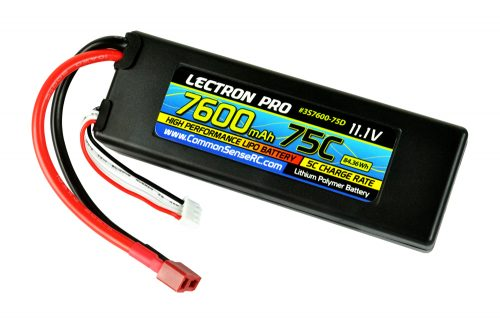
\includegraphics[width=0.9\linewidth]{battery.jpg}
	\caption{LiPo baterie \cite{dojo}}
	\label{fig:battery.jpg}
\end{figure}

\chapter[Fyzika letu dron]{Fyzika letu dronu}
K zajištění letu kvadrokoptéry je nezbytné, aby byla schopna vykonávat tři základní typy pohybu: vertikální pohyb, laterální pohyb a rotační pohyb. Každý z těchto pohybů lze realizovat prostřednictvím čtyř rotorů kvadrokoptéry.

\section[Vertikální pohyb]{Vertikální pohyb}
Newtonův třetí zákon pohybu stanovuje, že každé akci odpovídá stejně velká, avšak opačně orientovaná, reakce. V případě kvadrokoptéry dochází při rotaci jejích rotorů k vytlačování vzduchu směrem dolů, což představuje akční sílu. Na základě uvedeného zákona musí existovat odpovídající reakční síla, která působí směrem vzhůru na kvadrokoptéru. Jakmile velikost této vztlakové síly převýší gravitační sílu působící na kvadrokoptéru, dojde k jejímu vertikálnímu pohybu směrem vzhůru.

\section[Laterální pohyb]{Laterální pohyb}
Pokud vztlaková síla působí kolmo vzhůru, kvadrokoptéra se pohybuje vertikálně. Pokud však působí pod úhlem, dochází i k laterálnímu pohybu. Tento jev nastává v důsledku rozkladu vztlakové síly, která působí na dron jak ve vertikálním, tak v horizontálním směru. To způsobuje pohyb kvadrokoptéry do stran nebo ve směru dopředu a dozadu.\\
Laterální pohyb je realizován změnou rychlosti otáčení rotorů. Zvýšení rychlosti dvou rotorů na jedné straně kvadrokoptéry vede k nerovnoměrnému rozložení vztlakové síly. Strana s rychleji rotujícími rotory generuje větší vztlak než opačná strana, což způsobí, že se nakloněná kvadrokoptéra pohybuje směrem k oblasti s nižším vztlakem.

\begin{figure}[H]
    \begin{subfigure}{0.45\linewidth}
        \centering
        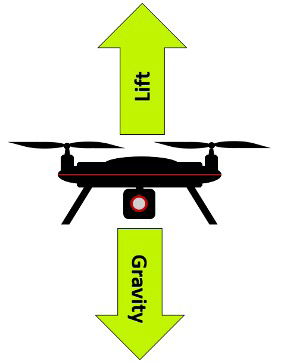
\includegraphics[width=0.6\linewidth]{vertical.png}
    \end{subfigure}
    \hfill
    \begin{subfigure}{0.45\linewidth}
        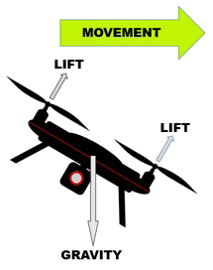
\includegraphics[width=0.6\linewidth]{lateral.png}
    \end{subfigure}
    \caption{Vertikální a laterální pohyb dronu \cite{nasa}}
    \label{fig:batteries}
\end{figure}

\section[Rotační pohyb]{Rotační pohyb}
Posledním typem pohybu kvadrokoptéry je rotace, která je výsledkem působení točivého momentu. Tento moment vzniká v důsledku otáčení rotorů, přičemž podle třetího Newtonova zákona se současně generuje síla opačného směru a stejné velikosti.\\
Točivý moment ovlivňuje kvadrokoptéru při rotaci rotorů, neboť každý jednotlivý rotor generuje svůj vlastní moment síly. Celkový točivý moment působící na kvadrokoptéru je součtem momentů všech čtyř rotorů. Pro eliminaci tohoto momentu se využívá konstrukční řešení, při němž se dva rotory otáčejí ve směru hodinových ručiček a dva v protisměru. Tyto momenty se vzájemně vyruší, čímž se eliminuje nekontrolovaná rotace kvadrokoptéry.\\

\begin{figure}[H]
	\centering
	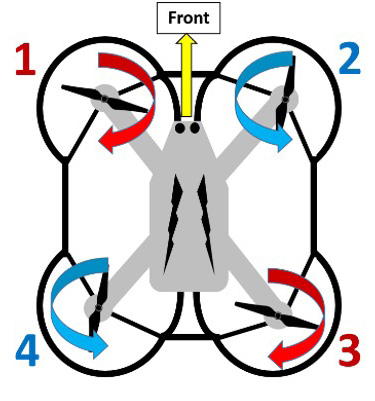
\includegraphics[width=0.4\linewidth]{rotational.png}
	\caption{Vyrušení točivých momentů rotorů \cite{nasa}}
	\label{fig:rotational.png}
\end{figure}

Točivý moment lze však také využít k řízené rotaci kvadrokoptéry. Pokud se například rotory 1 a 3 otáčejí rychleji než rotory 2 a 4, výsledný moment síly proti směru hodinových ručiček převáží nad momentem síly ve směru hodinových ručiček, což způsobí rotaci kvadrokoptéry proti směru hodinových ručiček. Naopak, pokud se rotory 2 a 4 otáčejí rychleji než rotory 1 a 3, kvadrokoptéra se začne otáčet ve směru hodinových ručiček. \cite{nasa} \cite{ca}
%%%%%%%%%%%%%% PRAKTICKÁ ČÁST %%%%%%%%%%%%%%%%%%	
\part{Konstrukce kvadrokoptéry} % název praktické části (nenechávejte název Praktická část)

\chapter[Součástky]{Součástky}
V této kapitole si ukážeme konkrétní použité součástky a vysvětlíme si jejich specifikace. Celý dron se skládá z rámu, motorů, ESC, rozvodné desky napájení a baterie. Řídicí jednotka se skládá z Arduina, nepájivého pole, Bluetooth modulu, modulu gyroskopu a akcelerometru. Většina těchto součástek byla zakoupena na internetovém obchodu Aliexpress.

\section[Rám]{Rám}
Při konstrukci dronu byl zvolen 3D tištěný rám pro jeho nízkou hmotnost a dostatečnou mechanickou odolnost. Využití 3D tisku umožnilo výrobu rámu s přesnými rozměry a vlastnostmi dle individuálních požadavků. Pro samotný tisk byl použit standardní materiál PLA, který se vyznačuje snadnou tisknutelností a přiměřenou pevností.\\
Model rámu vznikl úpravou existujícího designu z platformy Thingiverse \cite{ram}. Tato stránka poskytuje veškeré potřebné modely pro 3D tisk, které jsou volně dostupné ke stažení a úpravě.\\
Jednotlivé části vytištěného rámu byly smontovány pomocí šroubů a matic.
\begin{figure}[H]
	\centering
	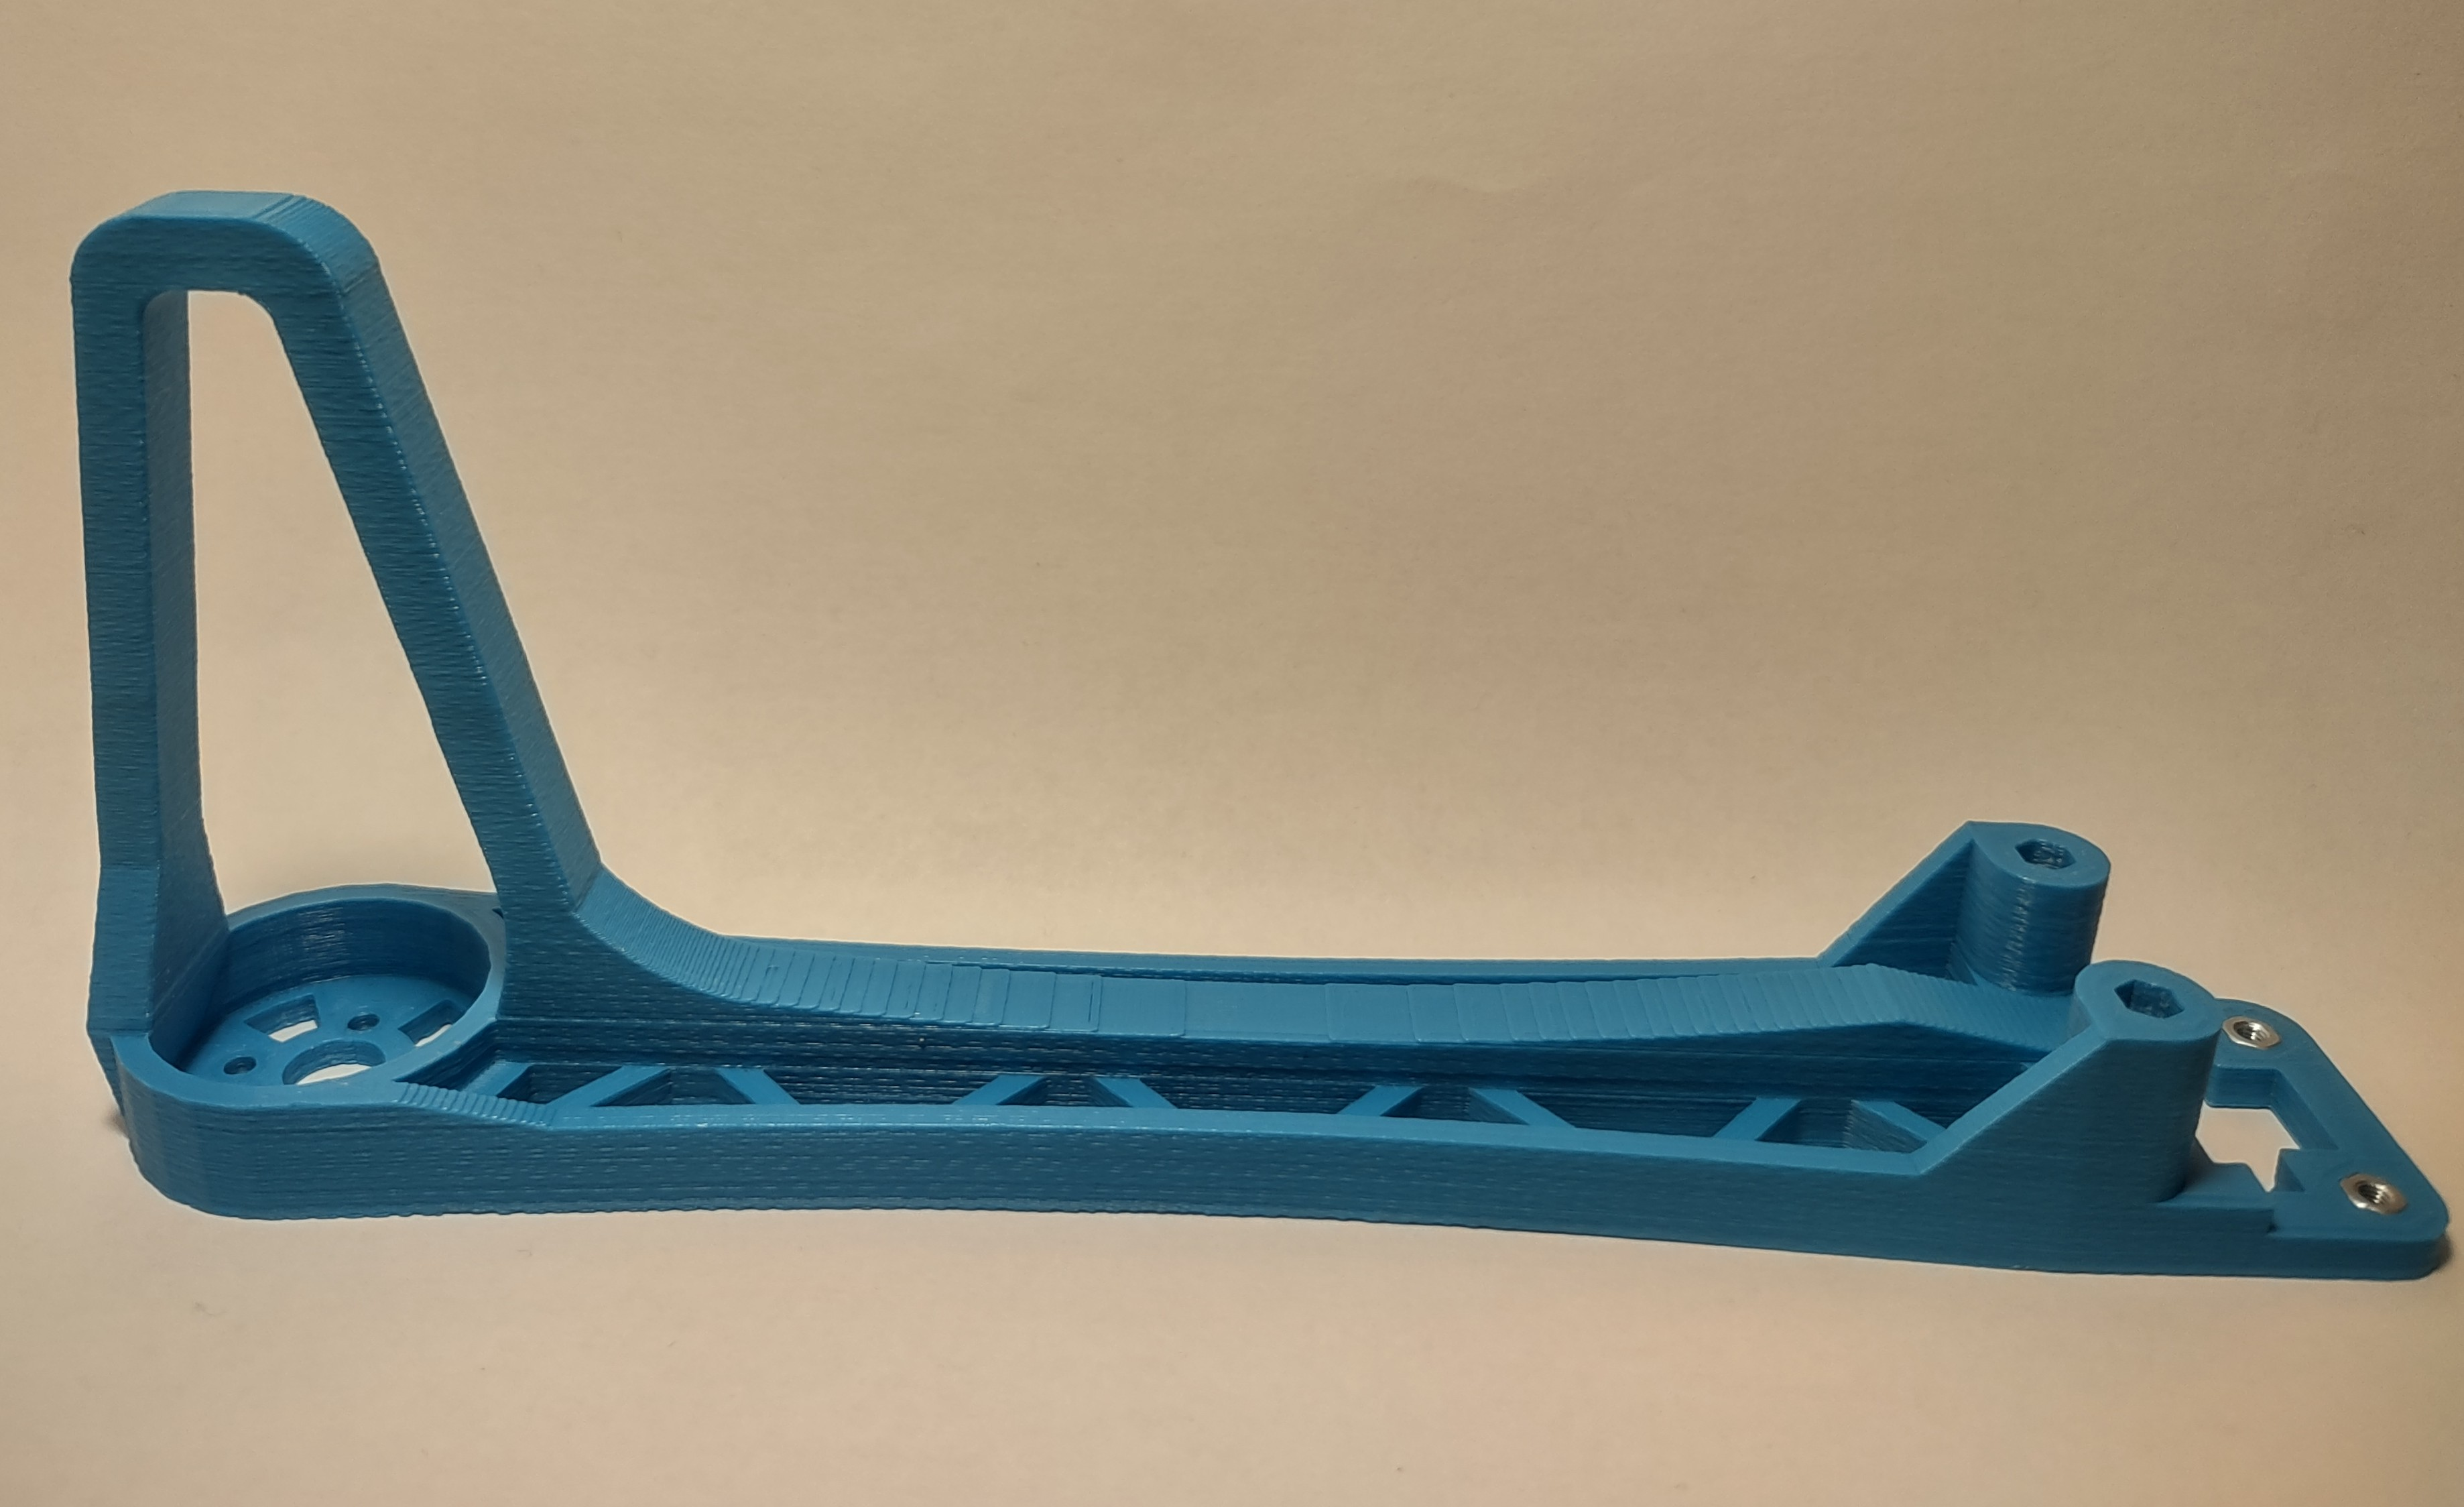
\includegraphics[width=0.75\linewidth]{ram2.jpg}
	\caption{Rameno rámu kvadrokoptéry}
	\label{fig:ram2.jpg}
\end{figure}

\section[Motory]{Motory}
Jako pohonná jednotka byl zvolen bezkartáčový motor 2212 920KV, který nabízí optimální rovnováhu mezi výkonem a spotřebou energie. U dronů se obecně preferují outrunner motory, které jsou díky své konstrukci efektivnější, poskytují vyšší točivý moment a lepší chladicí vlastnosti.\\
Hodnota KV udává počet otáček motoru za minutu (RPM) na jeden volt napájecího napětí. To znamená, že například motor 2212 920KV při napětí 1V dosáhne přibližně 920 ot./min, při 2V to bude 1840 ot./min atd.\\
První uvedené číslo v označení motoru (2212) udává jeho rozměry. První dvě číslice (22) udávají průměr statoru a druhé dvě číslice (12) označují výšku statoru v milimetrech.\\
\begin{figure}[H]
	\centering
	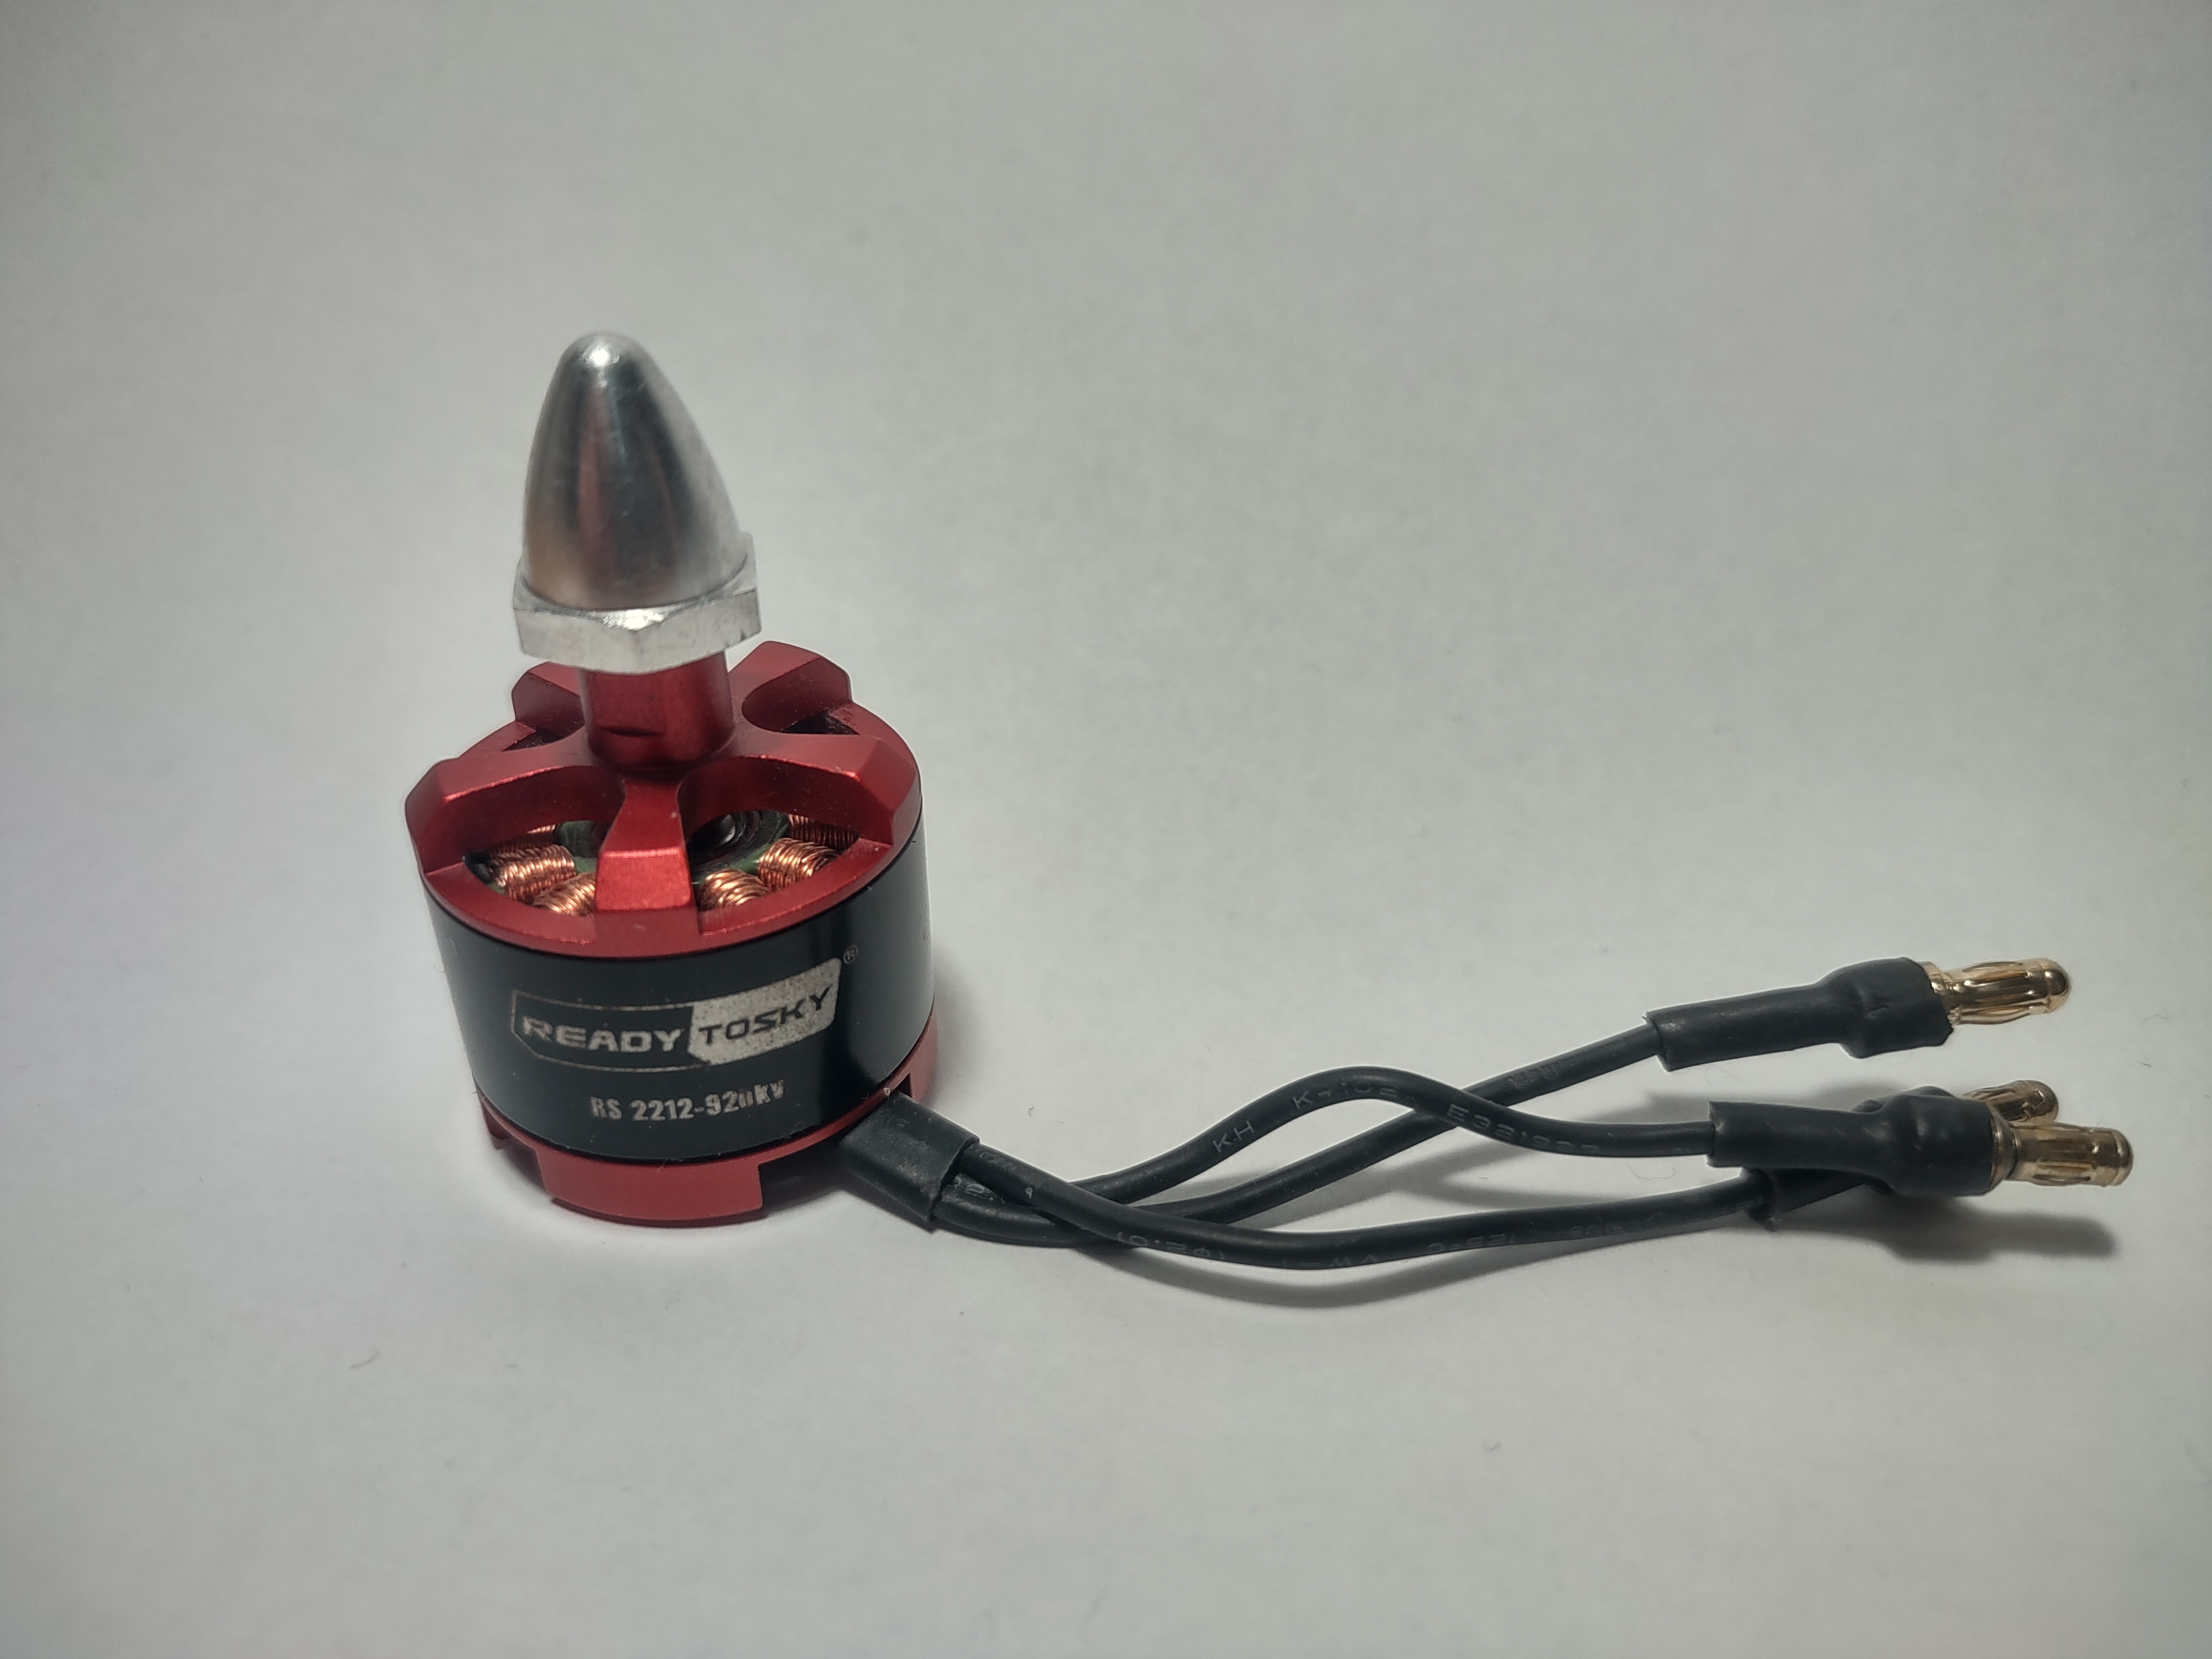
\includegraphics[width=0.7\linewidth]{motor.jpg}
	\caption{CCW bezkartáčový motor 2212 920KV}
	\label{fig:motor.jpg}
\end{figure}
V neposlední řadě je důležité dbát na správnou orientaci závitu tak, aby se utahování vrtule vždy provádělo proti směru otáčení motoru. Toto řešení je klíčové z hlediska bezpečnosti, protože zabraňuje uvolnění vrtule při prudkém zpomalení nebo zastavení motoru. Pro stabilizaci letu je nutné, aby byly použity dva motory s pravotočivou rotací (CW - Clockwise) a dva s levotočivou rotací (CCW - Counterclockwise). \cite{ol}\\

\section[Vrtule]{Vrtule}
Zvolené vrtule nesou označení 1045, kde první dvě číslice označují průměr vrtule v palcích a poslední dvě číslice představují stoupání vrtule v palcích. Stoupání vrtule (propeller pitch) určuje vzdálenost, kterou vrtule urazí při jednom otočení za ideálních podmínek. Vyšší stoupání znamená větší objem vzduchu přemístěného směrem dolů během rotace, což zvyšuje tah, ale zároveň zvyšuje aerodynamický odpor a zatížení motoru. Princip lze přirovnat ke závitu šroubu, kde stoupání určuje hloubku zavrtání za otáčku. Existují dvě varianty vrtulí, podle jejich směru točení (CW a CCW).\\

\section[ESC]{ESC}
Brushless motory vyžadují třífázové napájení, což je poměrně složitý proces, který zajišťuje vestavěný mikrořadič v ESC. Z našeho pohledu stačí do ESC přivést napájecí proud a prostřednictvím signálního vodiče mu sdělit, jakou rychlostí se má motor otáčet.\\
Je důležité zajistit, aby ESC bylo kompatibilní s daným bezkartáčovým motorem. Klíčovými parametry jsou maximální napětí a proud, které ESC zvládne. Pro správnou funkci je také nutné ESC spájet s rozvodnou deskou napájení, která rozvádí napětí z baterie ke všem komponentům.
\begin{figure}[H]
	\centering
	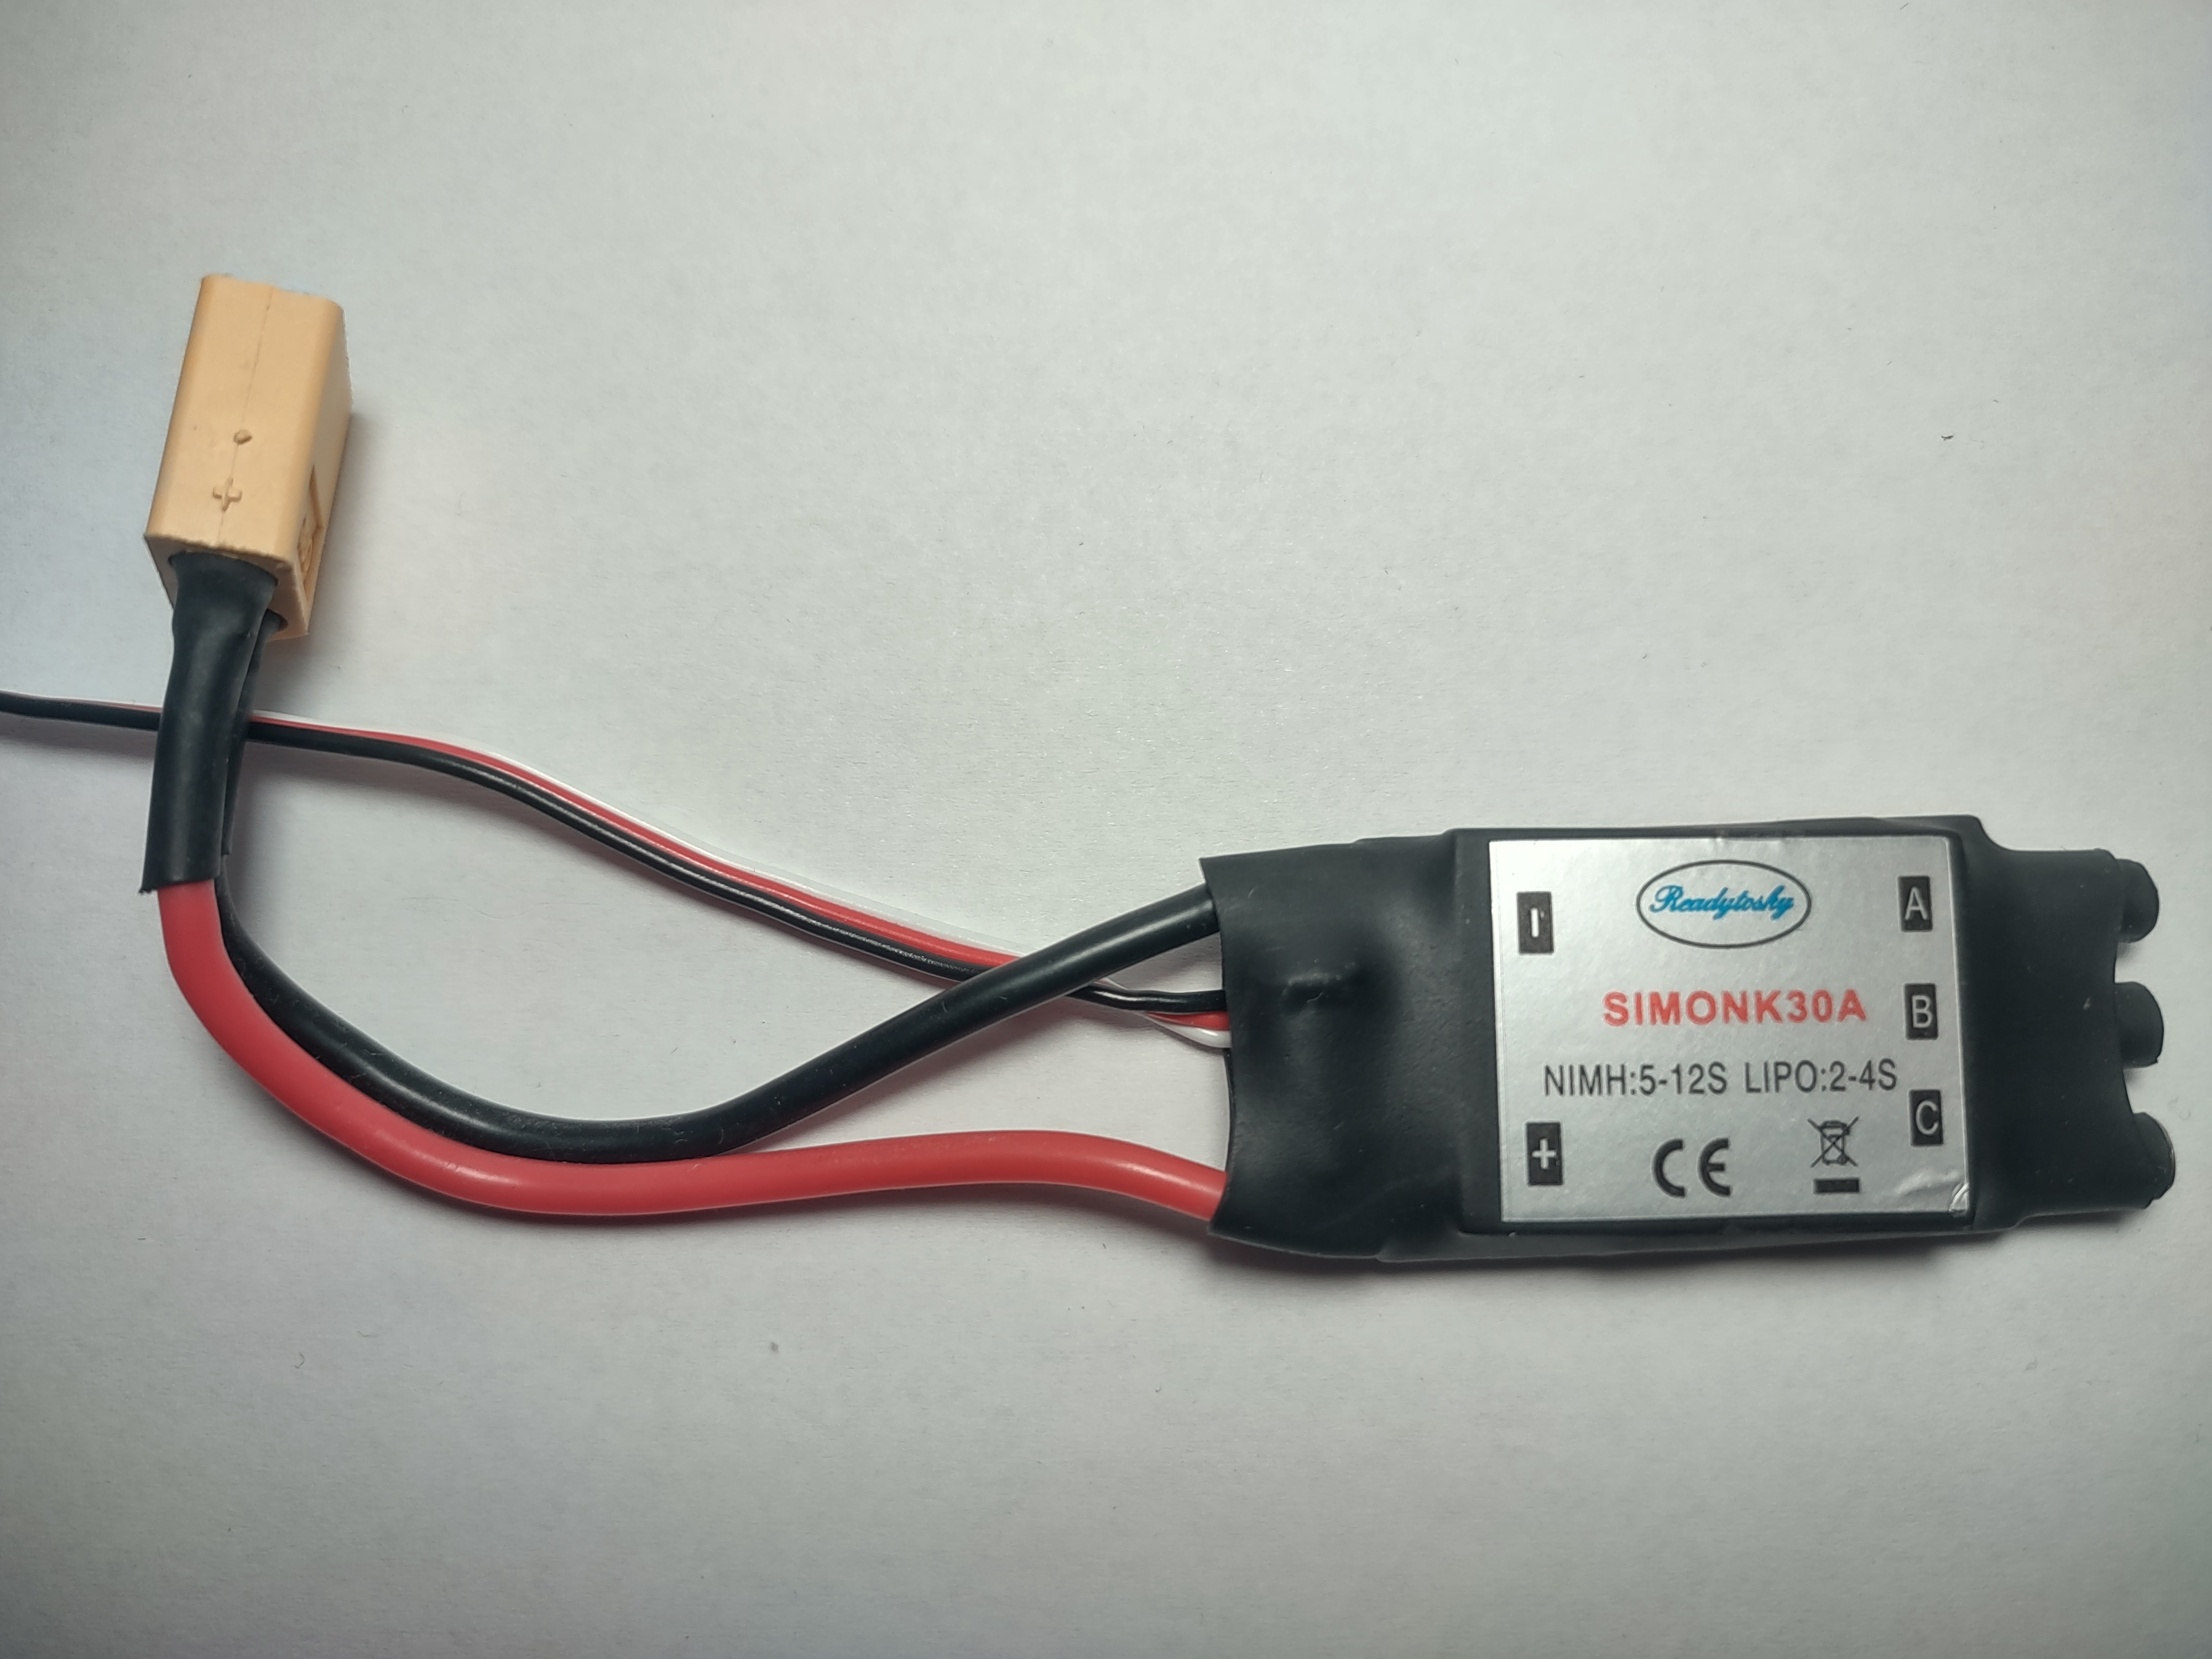
\includegraphics[width=0.6\linewidth]{esc.jpg}
	\caption{ESC pro bezkartáčové motory}
	\label{fig:esc.jpg}
\end{figure}

\section{Rozvodná deska napájení}
Rozvodná deska napájení (PDB) slouží k distribuci energie z baterie do všech komponent. Všechny čtyři ESC jsou k této desce připájeny a baterie je k ní připojena přes bezpečný napájecí konektor.

\section[Baterie]{Baterie}
Jedná se o zdroj veškeré energie pro dron. V této práci byla vybrána baterie se specifikací LiPo 2200mAh 14.8V 30C 4S1P.
\begin{figure}[H]
	\centering
	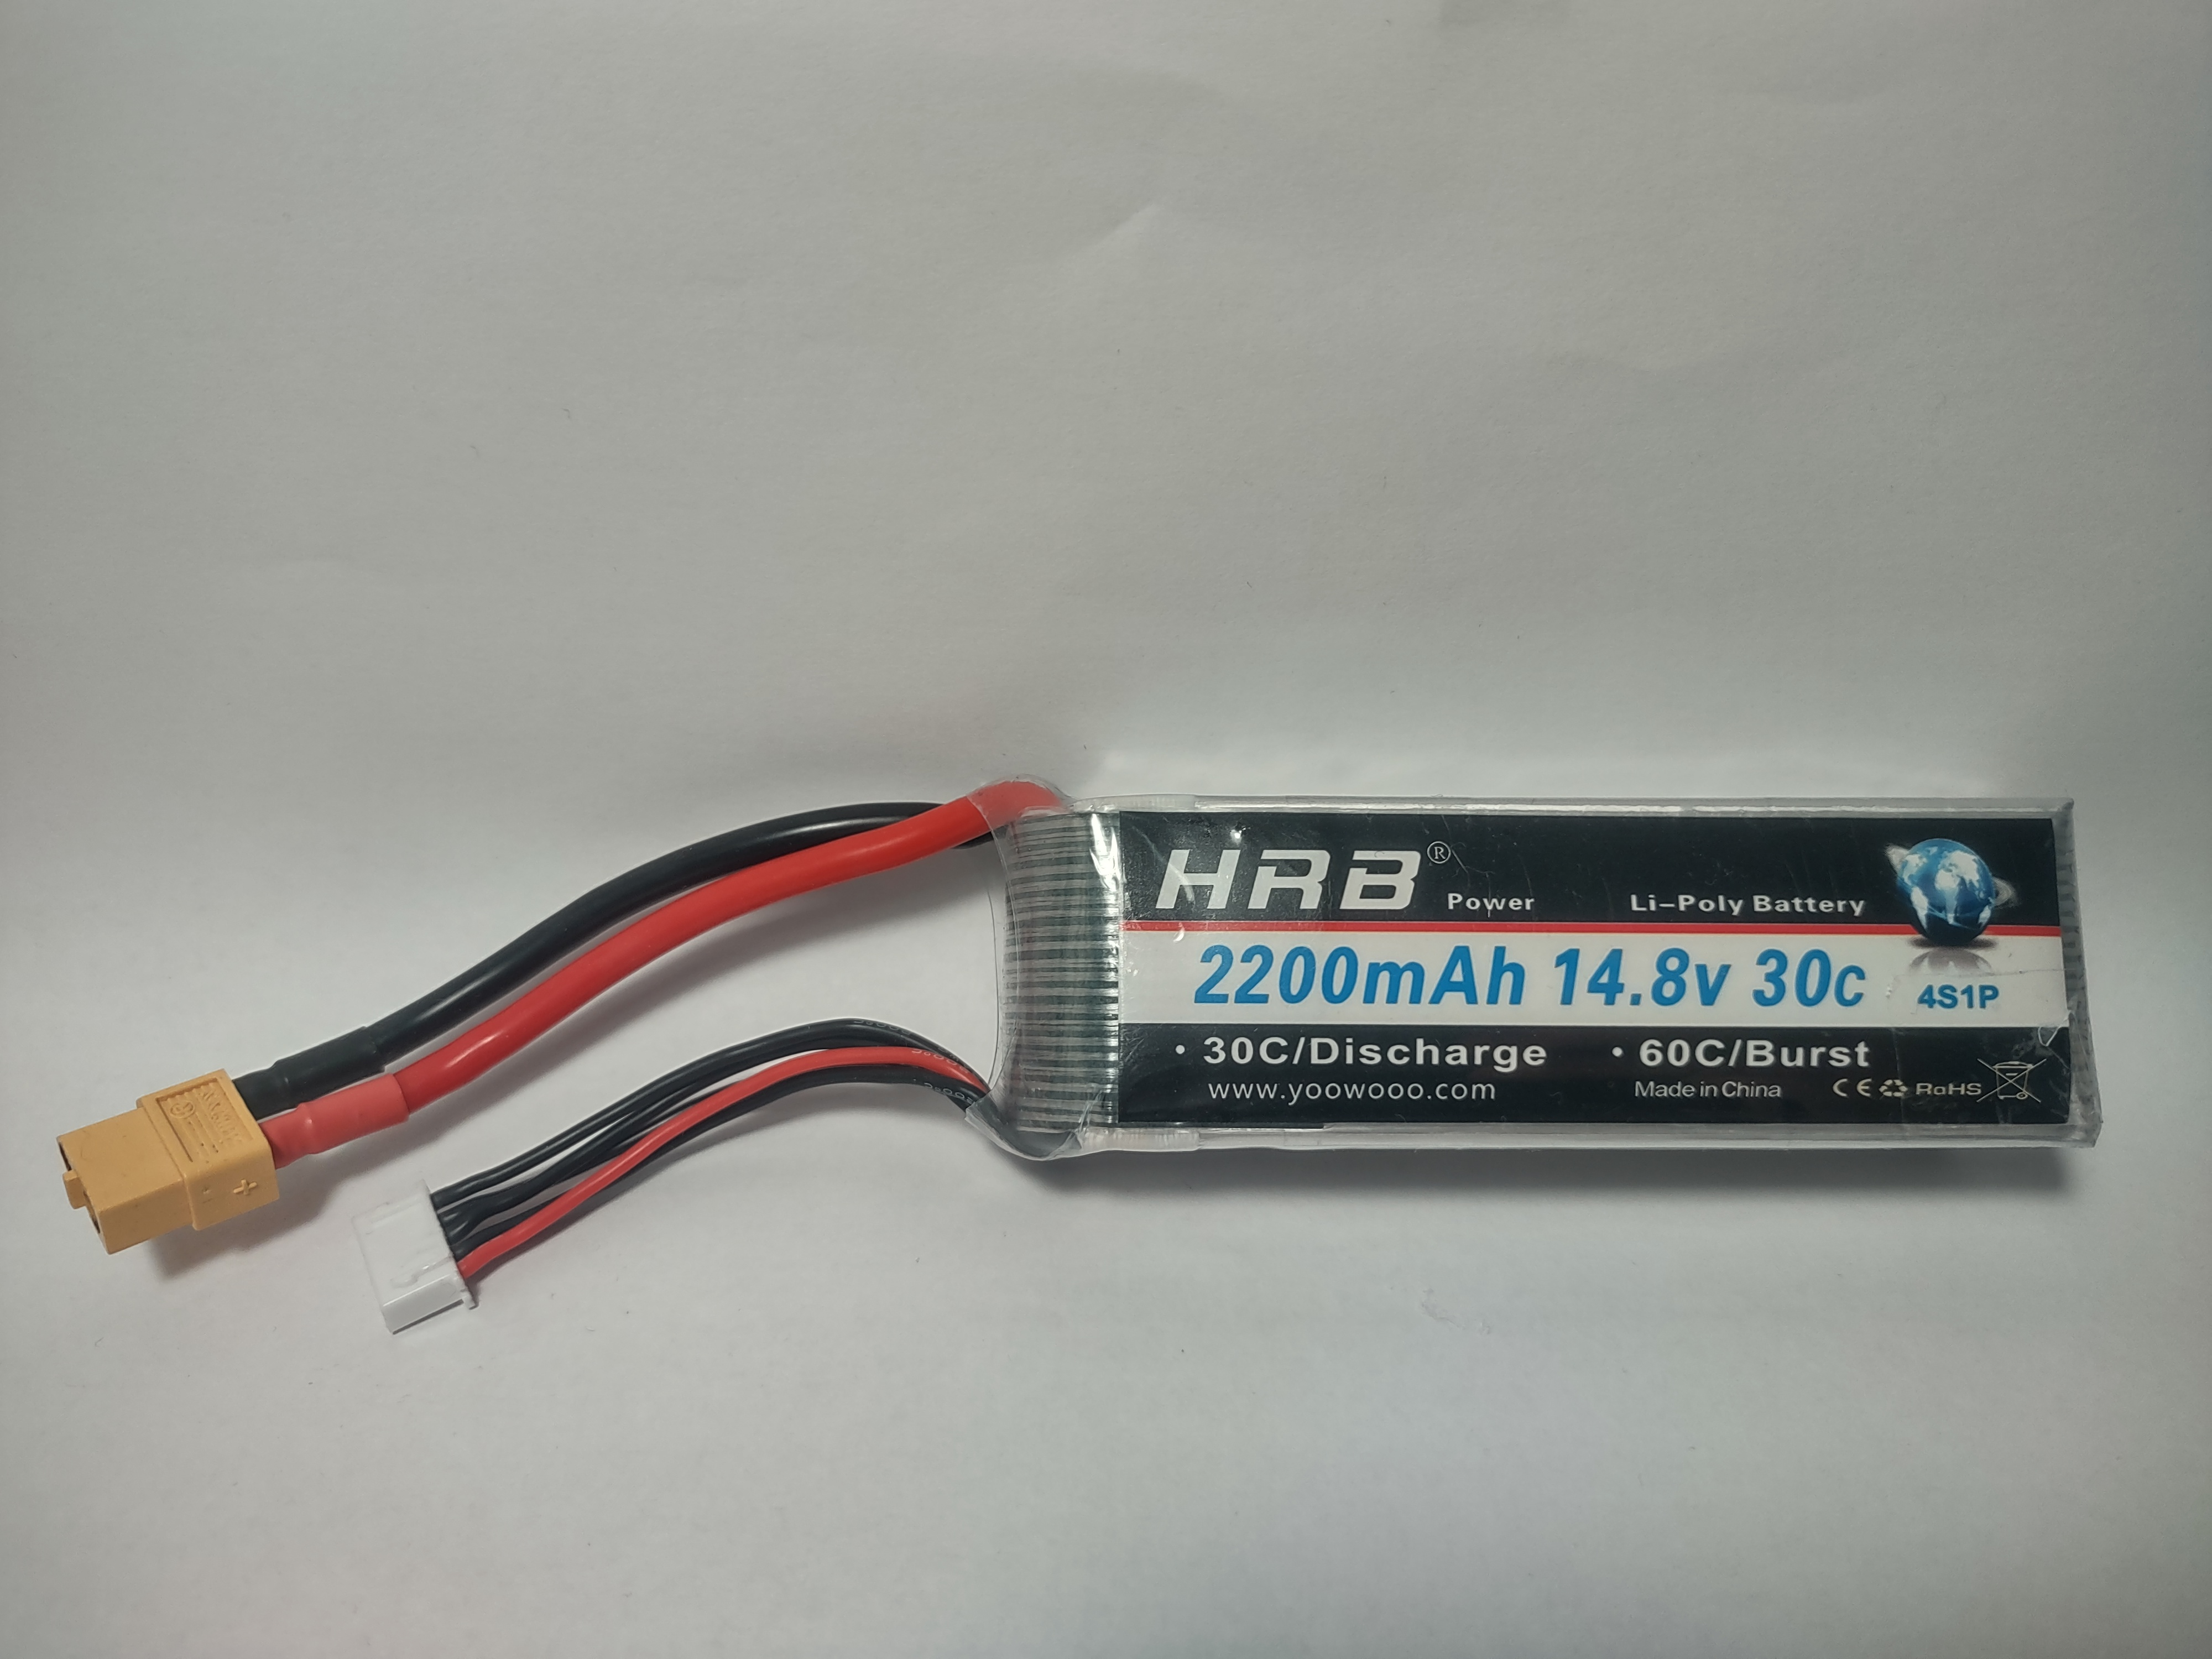
\includegraphics[width=0.6\linewidth]{battery2.jpg}
	\caption{LiPo baterie 2200mAh 14.8V 30C 4S1P}
	\label{fig:battery2.jpg}
\end{figure}
Začněme částí 4S. Bateriový pack je složen z jednotlivých malých bateriových článků. Jeden LiPo článek má 4,2 V za předpokladu, že je plně nabitý. Označení 4S značí, že čtyři články jsou zapojeny sériově, což znamená, že výsledné napětí baterie se sčítá. Napětí celého, plně nabitého, bateriového packu tedy činí 16,8 V.\\
Hodnota 2200mAh označuje celkovou kapacitu baterie, což znamená, že při odběru 2,2 A by baterie měla teoreticky vydržet jednu hodinu.\\
Posledním parametrem je C-rating, který udává maximální proud, který je baterie schopna dodat. Maximální proud lze vypočítat jako C-rating × kapacita v Ah:
\[
30C \times 2.2\,\text{Ah} = 66\,\text{A}
\]
Tato hodnota představuje trvalý vybíjecí proud, který může baterie bezpečně poskytovat. Některé baterie mají také burst rating, kdy krátkodobě mohou dodat ještě vyšší proud, například dvojnásobek této hodnoty.

\section[Arduino]{Arduino}
Arduino je programovatelný mikrořadič umožňující připojení dalších komponent pro specifické aplikace. Pro tento projekt byla zvolena varianta Arduino UNO, a to především díky vysokému počtu připojovacích pinů a jednoduché manipulaci. Arduino zde plní funkci řídicí jednotky (flight controlleru), která na základě vstupních dat, získaných prostřednictvím Bluetooth modulu a akcelerometru, provádí výpočty potřebné k regulaci motorů. Zařízení nevyžaduje samostatný napájecí zdroj, neboť je napájeno přímo z motorů.

\section[Bluetooth modul]{Bluetooth modul}
Bluetooth modul HC-05 je bezdrátový komunikační modul umožňující obousměrný přenos dat mezi Arduinem a externím zařízením. Pro tento projekt byl zvolen HC-05, díky své kompatibilitě a jednoduché implementaci sériové komunikace prostřednictvím protokolu UART. Modul umožňuje bezdrátové ovládání a přenos řídicích signálů mezi uživatelským rozhraním mobilní aplikace a řídicí jednotkou letu. HC-05 pracuje ve frekvenčním pásmu 2,4 GHz s maximálním dosahem přibližně 10–20 metrů, což je pro tento projekt dostačující. Přenosová rychlost modulu může dosahovat až 1 Mb/s. 
\begin{figure}[H]
	\centering
	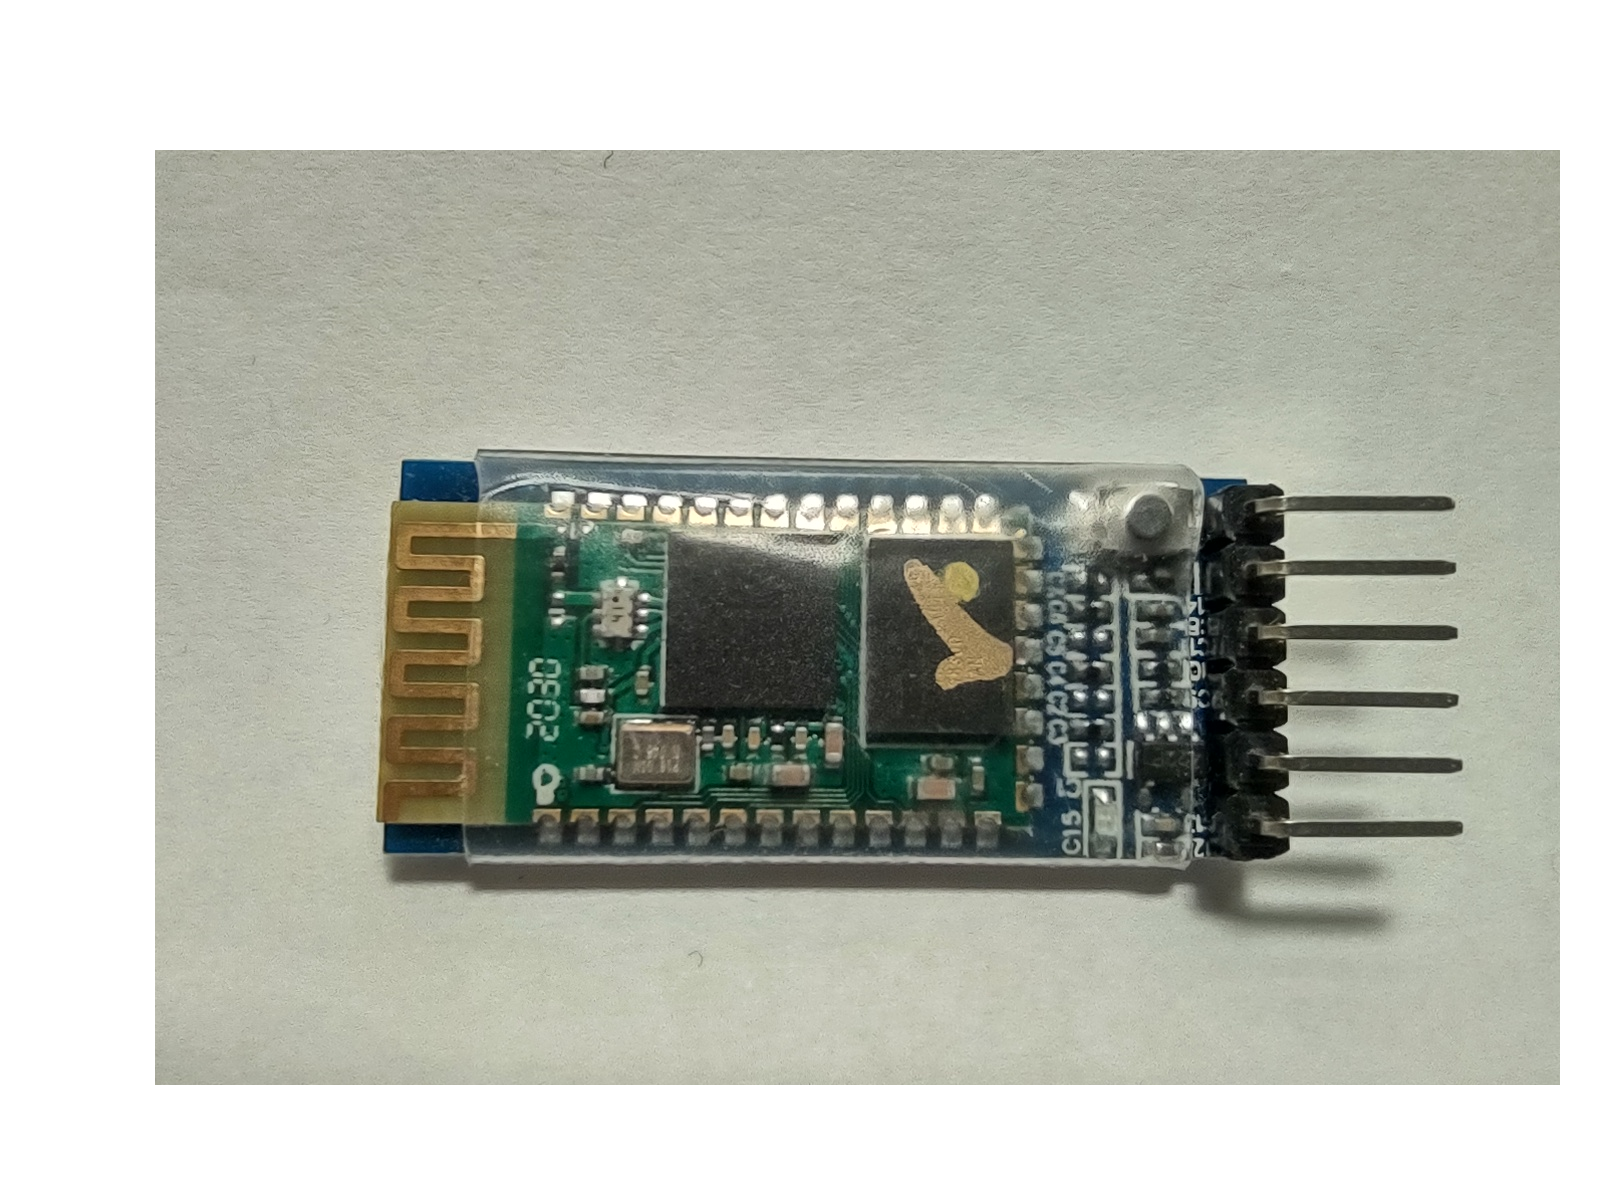
\includegraphics[width=0.55\linewidth]{hc-05.png}
	\caption{Bluetooth modul HC-05}
	\label{fig:hc-05.png}
\end{figure}
\section[Akcelerometr a gyroskop]{Akcelerometr a gyroskop}
MPU6050 je měřicí jednotka složená ze tříosého gyroskopu a tříosého akcelerometru, což umožňuje komplexní měření pohybu a orientace v prostoru. Pro tento projekt byl zvolen modul MPU6050 díky jeho vysoké přesnosti a kompaktním rozměrům. Modul poskytuje klíčová data o náklonu, zrychlení a úhlové rychlosti, která jsou využívána řídicí jednotkou při výpočtu stabilizačních algoritmů a optimalizaci řízení motorů.
\begin{figure}[H]
	\centering
	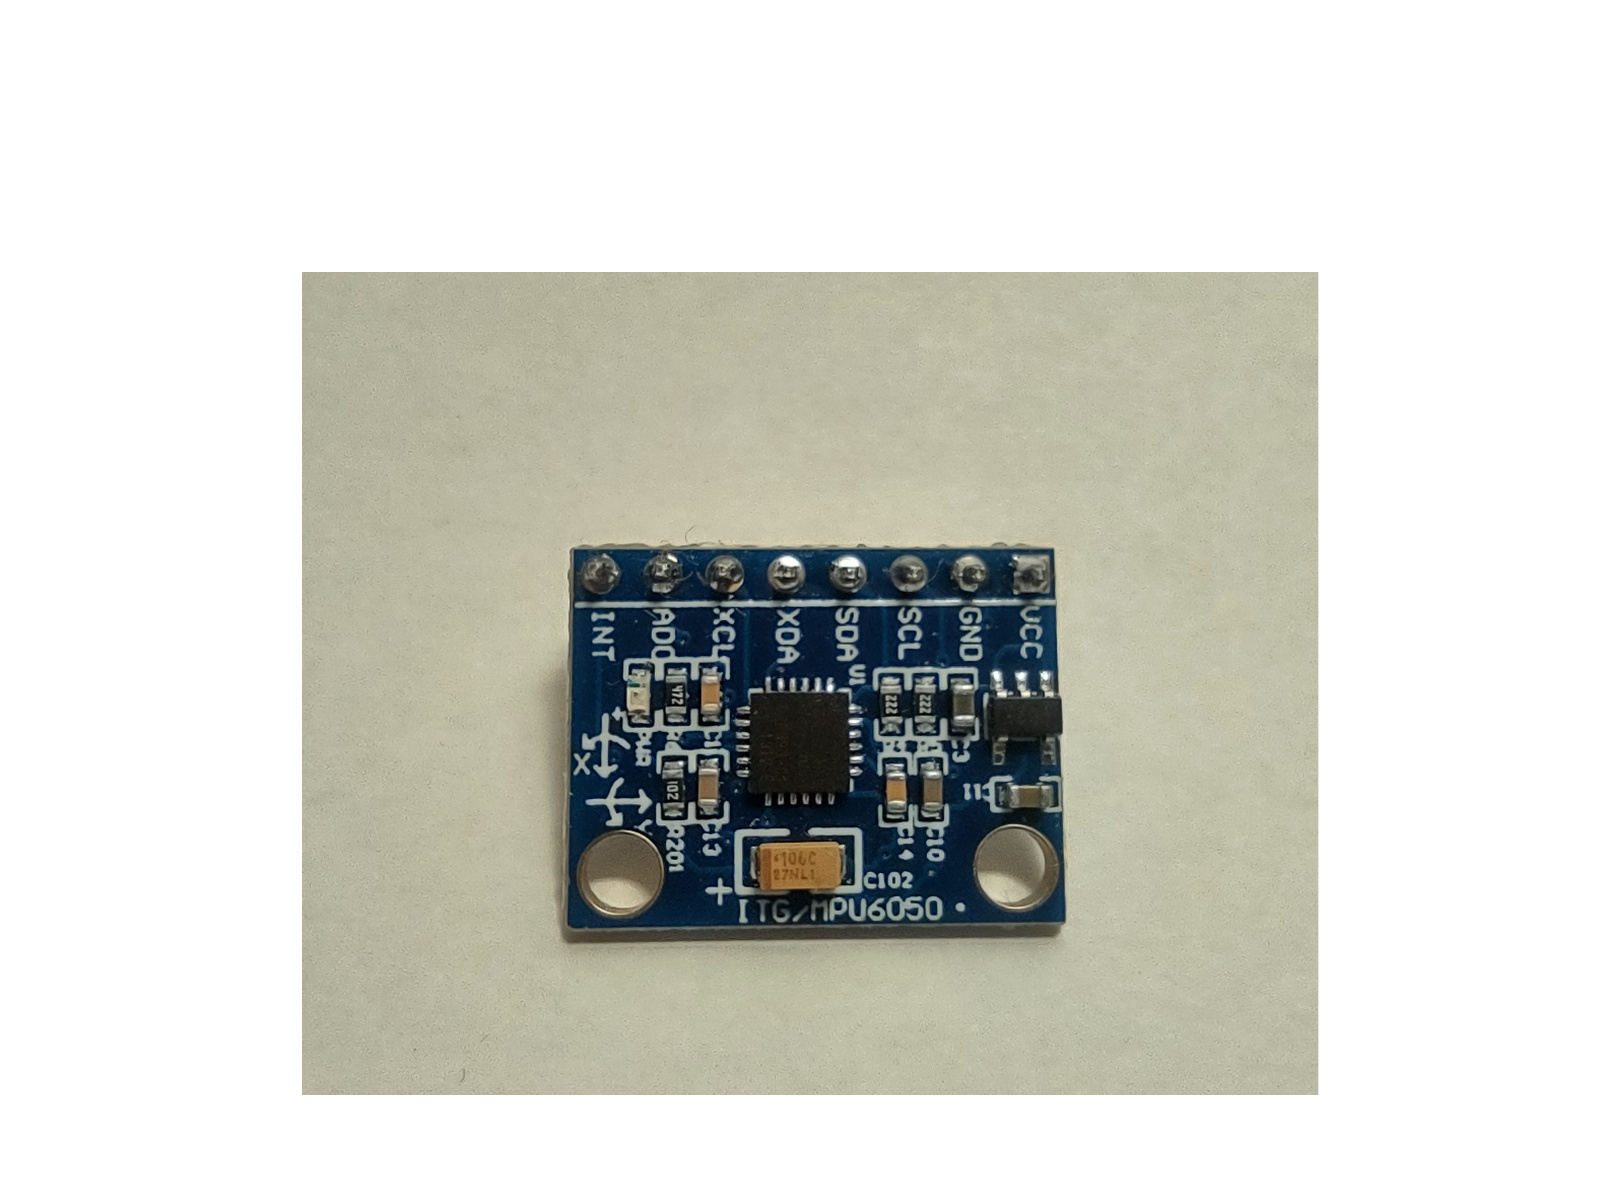
\includegraphics[width=0.55\linewidth]{mpu6050.png}
	\caption{Akcelerometr a gyroskop MPU6050}
	\label{fig:hc-05.png}
\end{figure}

\chapter[Průběh Konstrukce]{Průběh Konstrukce}
Prvním krokem při konstrukci dronu bylo vytvoření jeho rámu pomocí 3D tisku. Po několika neúspěšných pokusech se podařilo úspěšně vytisknout jednotlivé součásti s požadovanou přesností a strukturální pevností. Do klíčových částí rámu byly zataveny kovové závitové vložky, které umožňují pevné uchycení komponent pomocí šroubů. Ty byly umístěny především v centrální části rámu, kde bylo nezbytné pevně připojit ramena ke středu rámu a na koncích ramen, kde dochází k upevnění motorů s vysokým tahem.\\
Dalším krokem byla instalace a zapojení napájecího systému. Jednotlivé napájecí vodiče motorů byly připájeny k rozvodové desce, která zajišťuje distribuci elektrické energie v celém zařízení. Stejným způsobem byl k rozvodové desce připojen hlavní napájecí kabel, přes který je k desce připojena baterie. Po dokončení byly motory rozmístěny na koncích ramen dronu tak, aby jejich směr otáčení odpovídal požadované konfiguraci letového systému.\\
Motory byly ke konstrukci připevněny pomocí šroubků, přičemž pro dodatečnou stabilizaci byly elektronické regulátory otáček (ESC) zajištěny pomocí instalačních pásků.\\
Po dokončení mechanické konstrukce dronu následoval klíčový krok, kterým je návrh a implementace řídicí jednotky (flight controlleru).
\begin{figure}[H]
	\centering
	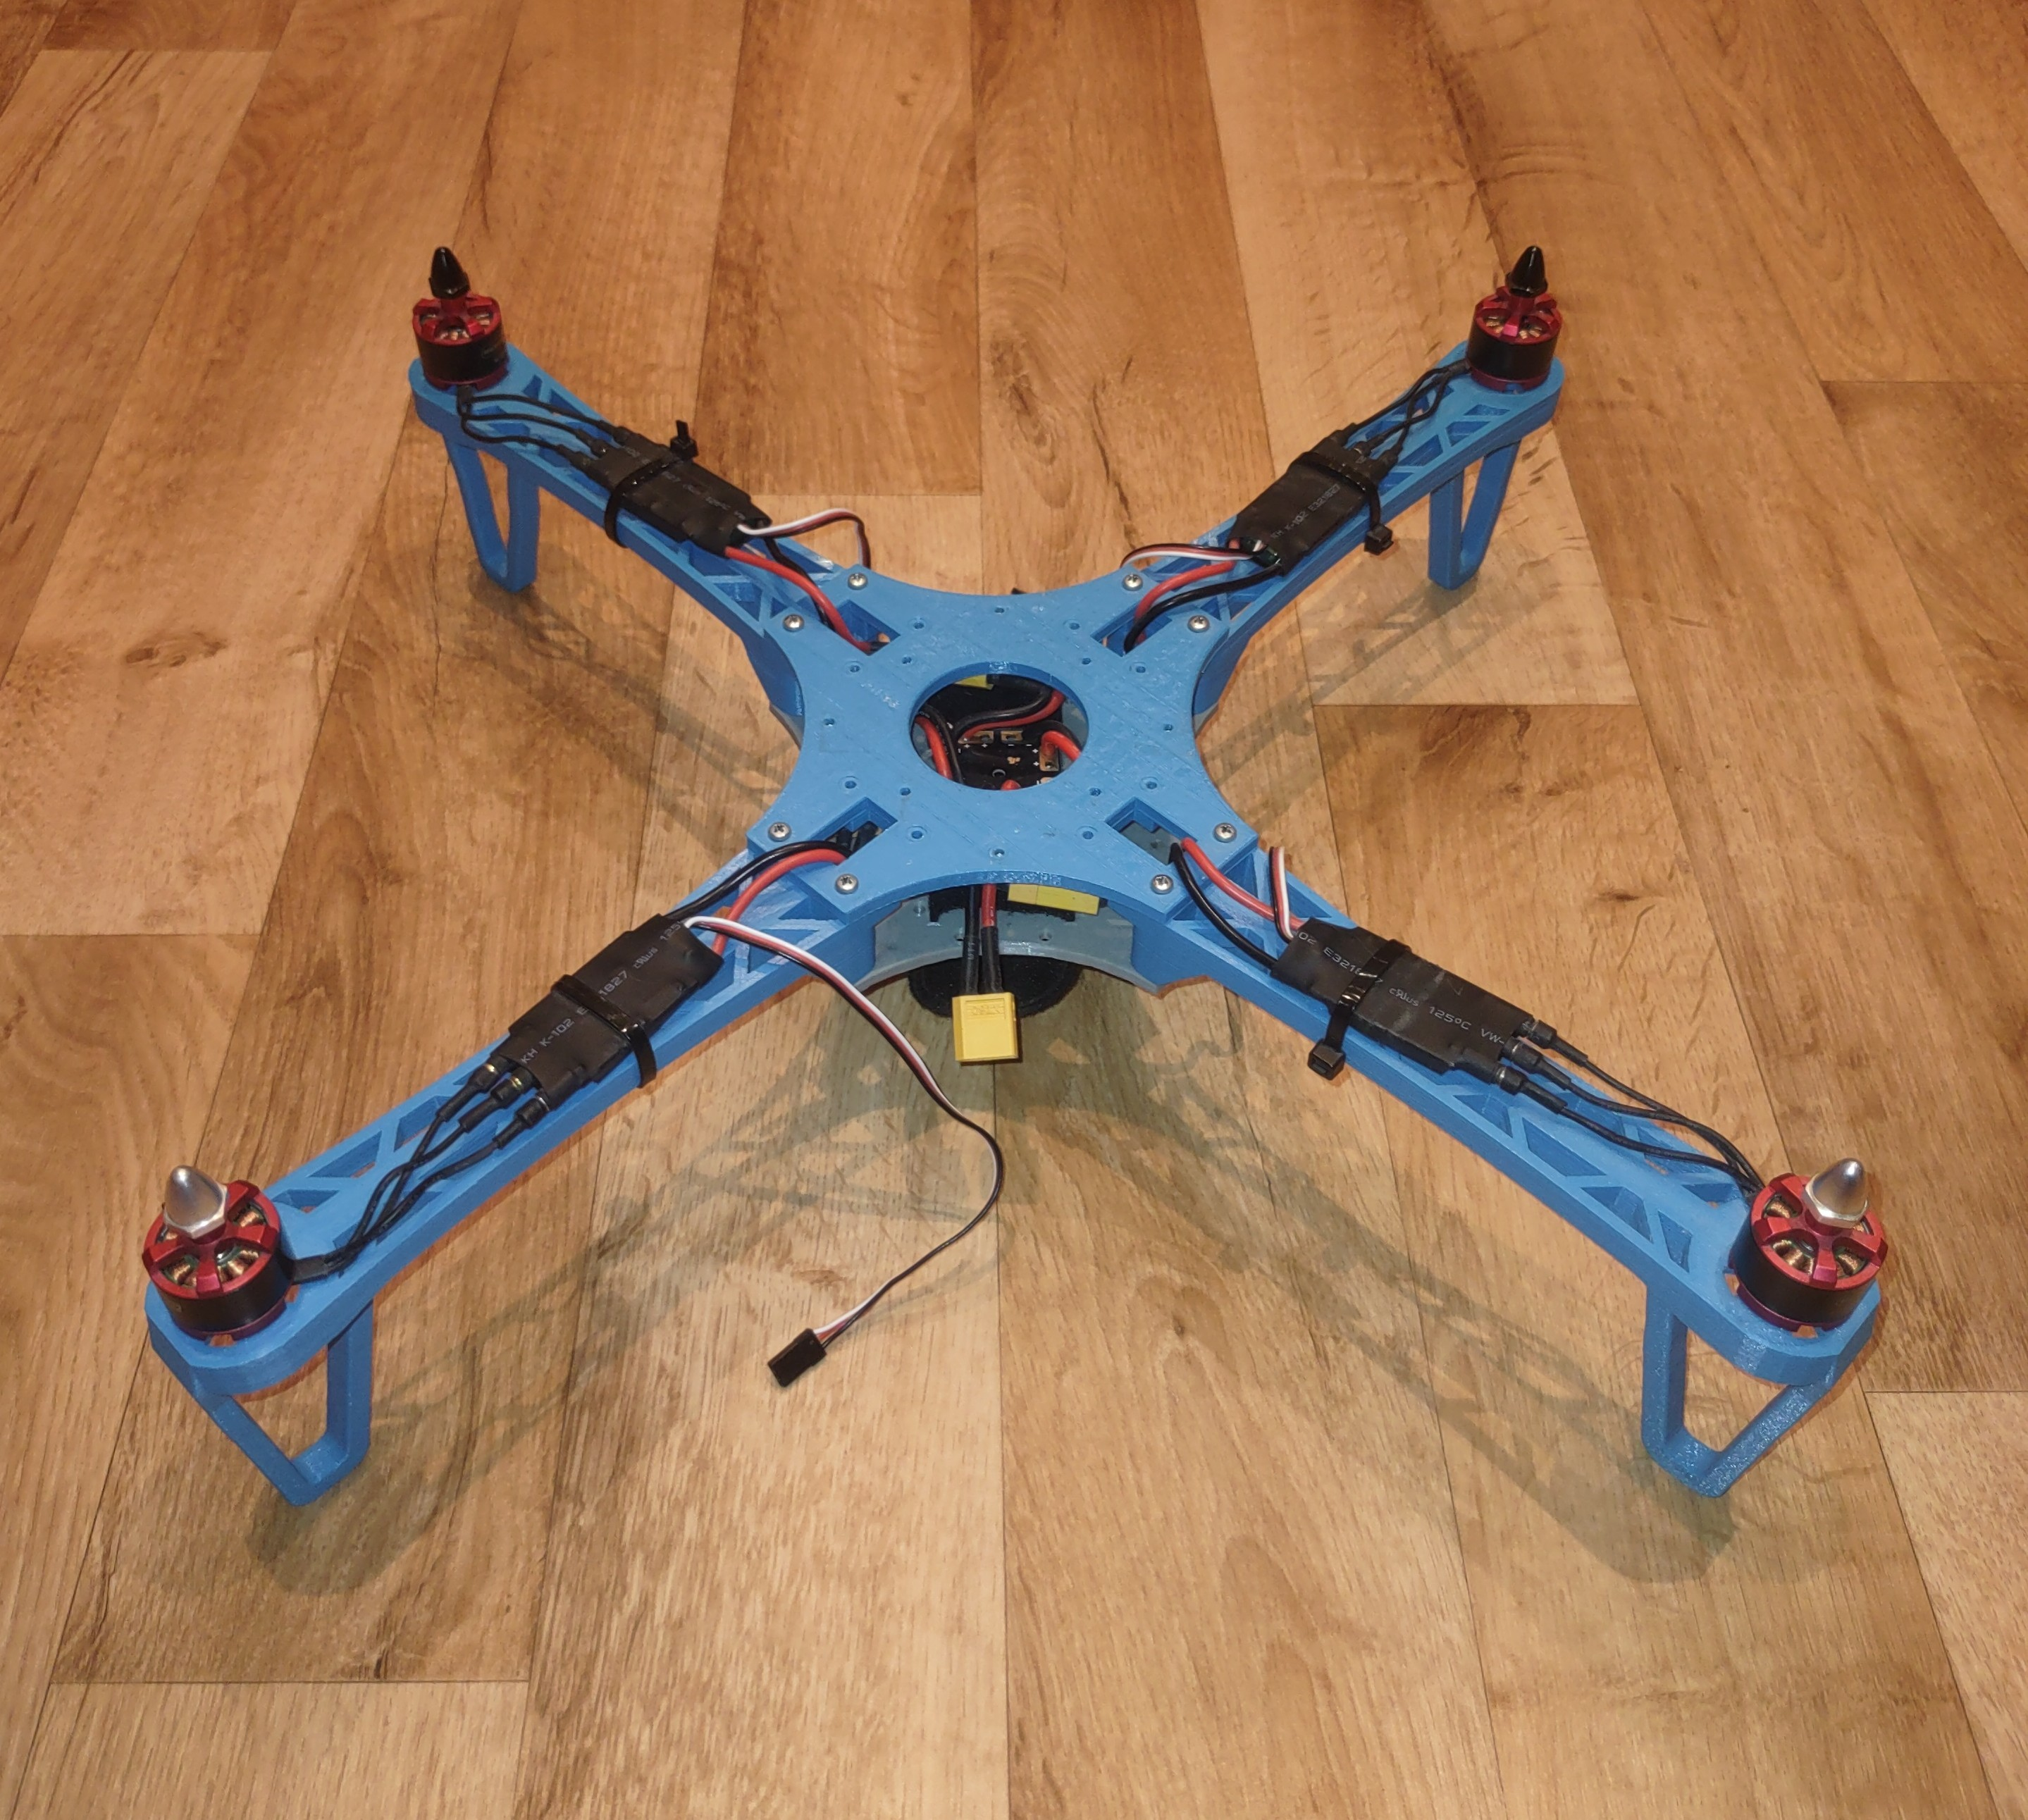
\includegraphics[width=0.75\linewidth]{zakladni-konstrukce.jpg}
	\caption{Základní konstrukce rámu s motory a ESC}
	\label{fig:zakladni-konstrukce.jpg}
\end{figure}

\chapter[Vývoj řídicí jednotky]{Vývoj řídicí jednotky}
%%% v obsahu se objeví jen to co je v hranatých závorkách
Hlavním hardwarem řídicí jednotky je Arduino UNO. Prvním krokem bylo připojení Bluetooth modulu HC-05 a modulu akcelerometru a gyroskopu MPU6050. Tyto komponenty byly propojeny s Arduinem pomocí vodičů a nepájivého kontaktního pole, které umožňuje flexibilní zapojení a případné úpravy obvodu.\\
Software pro Arduino byl vytvořen v prostředí Arduino IDE, které je speciálně uzpůsobeno pro vývoj programů pro mikrořadič Arduino. Celý kód je nápsán v programovacím jazyce C++.\\
Mimo software pro řídicí jednotku bylo nutné vyvinout mobilní aplikaci, která umožňuje ovládání dronu prostřednictvím technologie Bluetooth. Pro tento účel byla využita aplikace Bluetooth Electronics \cite{be}, která poskytuje širokou škálu přizpůsobitelných tlačítek a ovládacích panelů. Tato aplikace rovněž umožňuje nastavení jednotlivých odesílaných příkazů odesílaných řídicí jednotce a zajišťuje propojení mezi mobilním zařízením a Bluetooth modulem dronu.\\
Profesionální drony jsou vybaveny pokročilým softwarem pro stabilizaci a automatickou korekci polohy. Konstrukčně realizovaný dron v této prací však funguje pouze na principu přímého ovládání motorů, přičemž neobsahuje stabilizační algoritmy. Výsledkem je vysoká nestabilita a značná náchylnost k pádu během letu. Implementace stabilizačního systému by vyžadovala složité programování, které by významně rozšířilo rozsah této maturitní práce.\\
Navržený dron je kompletně zhotoven po hardwarové stránce, přičemž zbývající vývoj pro stabilizovaný let se týká výhradně implementace softwarového stabilizačního systému v Arduinu.
\begin{figure}[H]
	\centering
	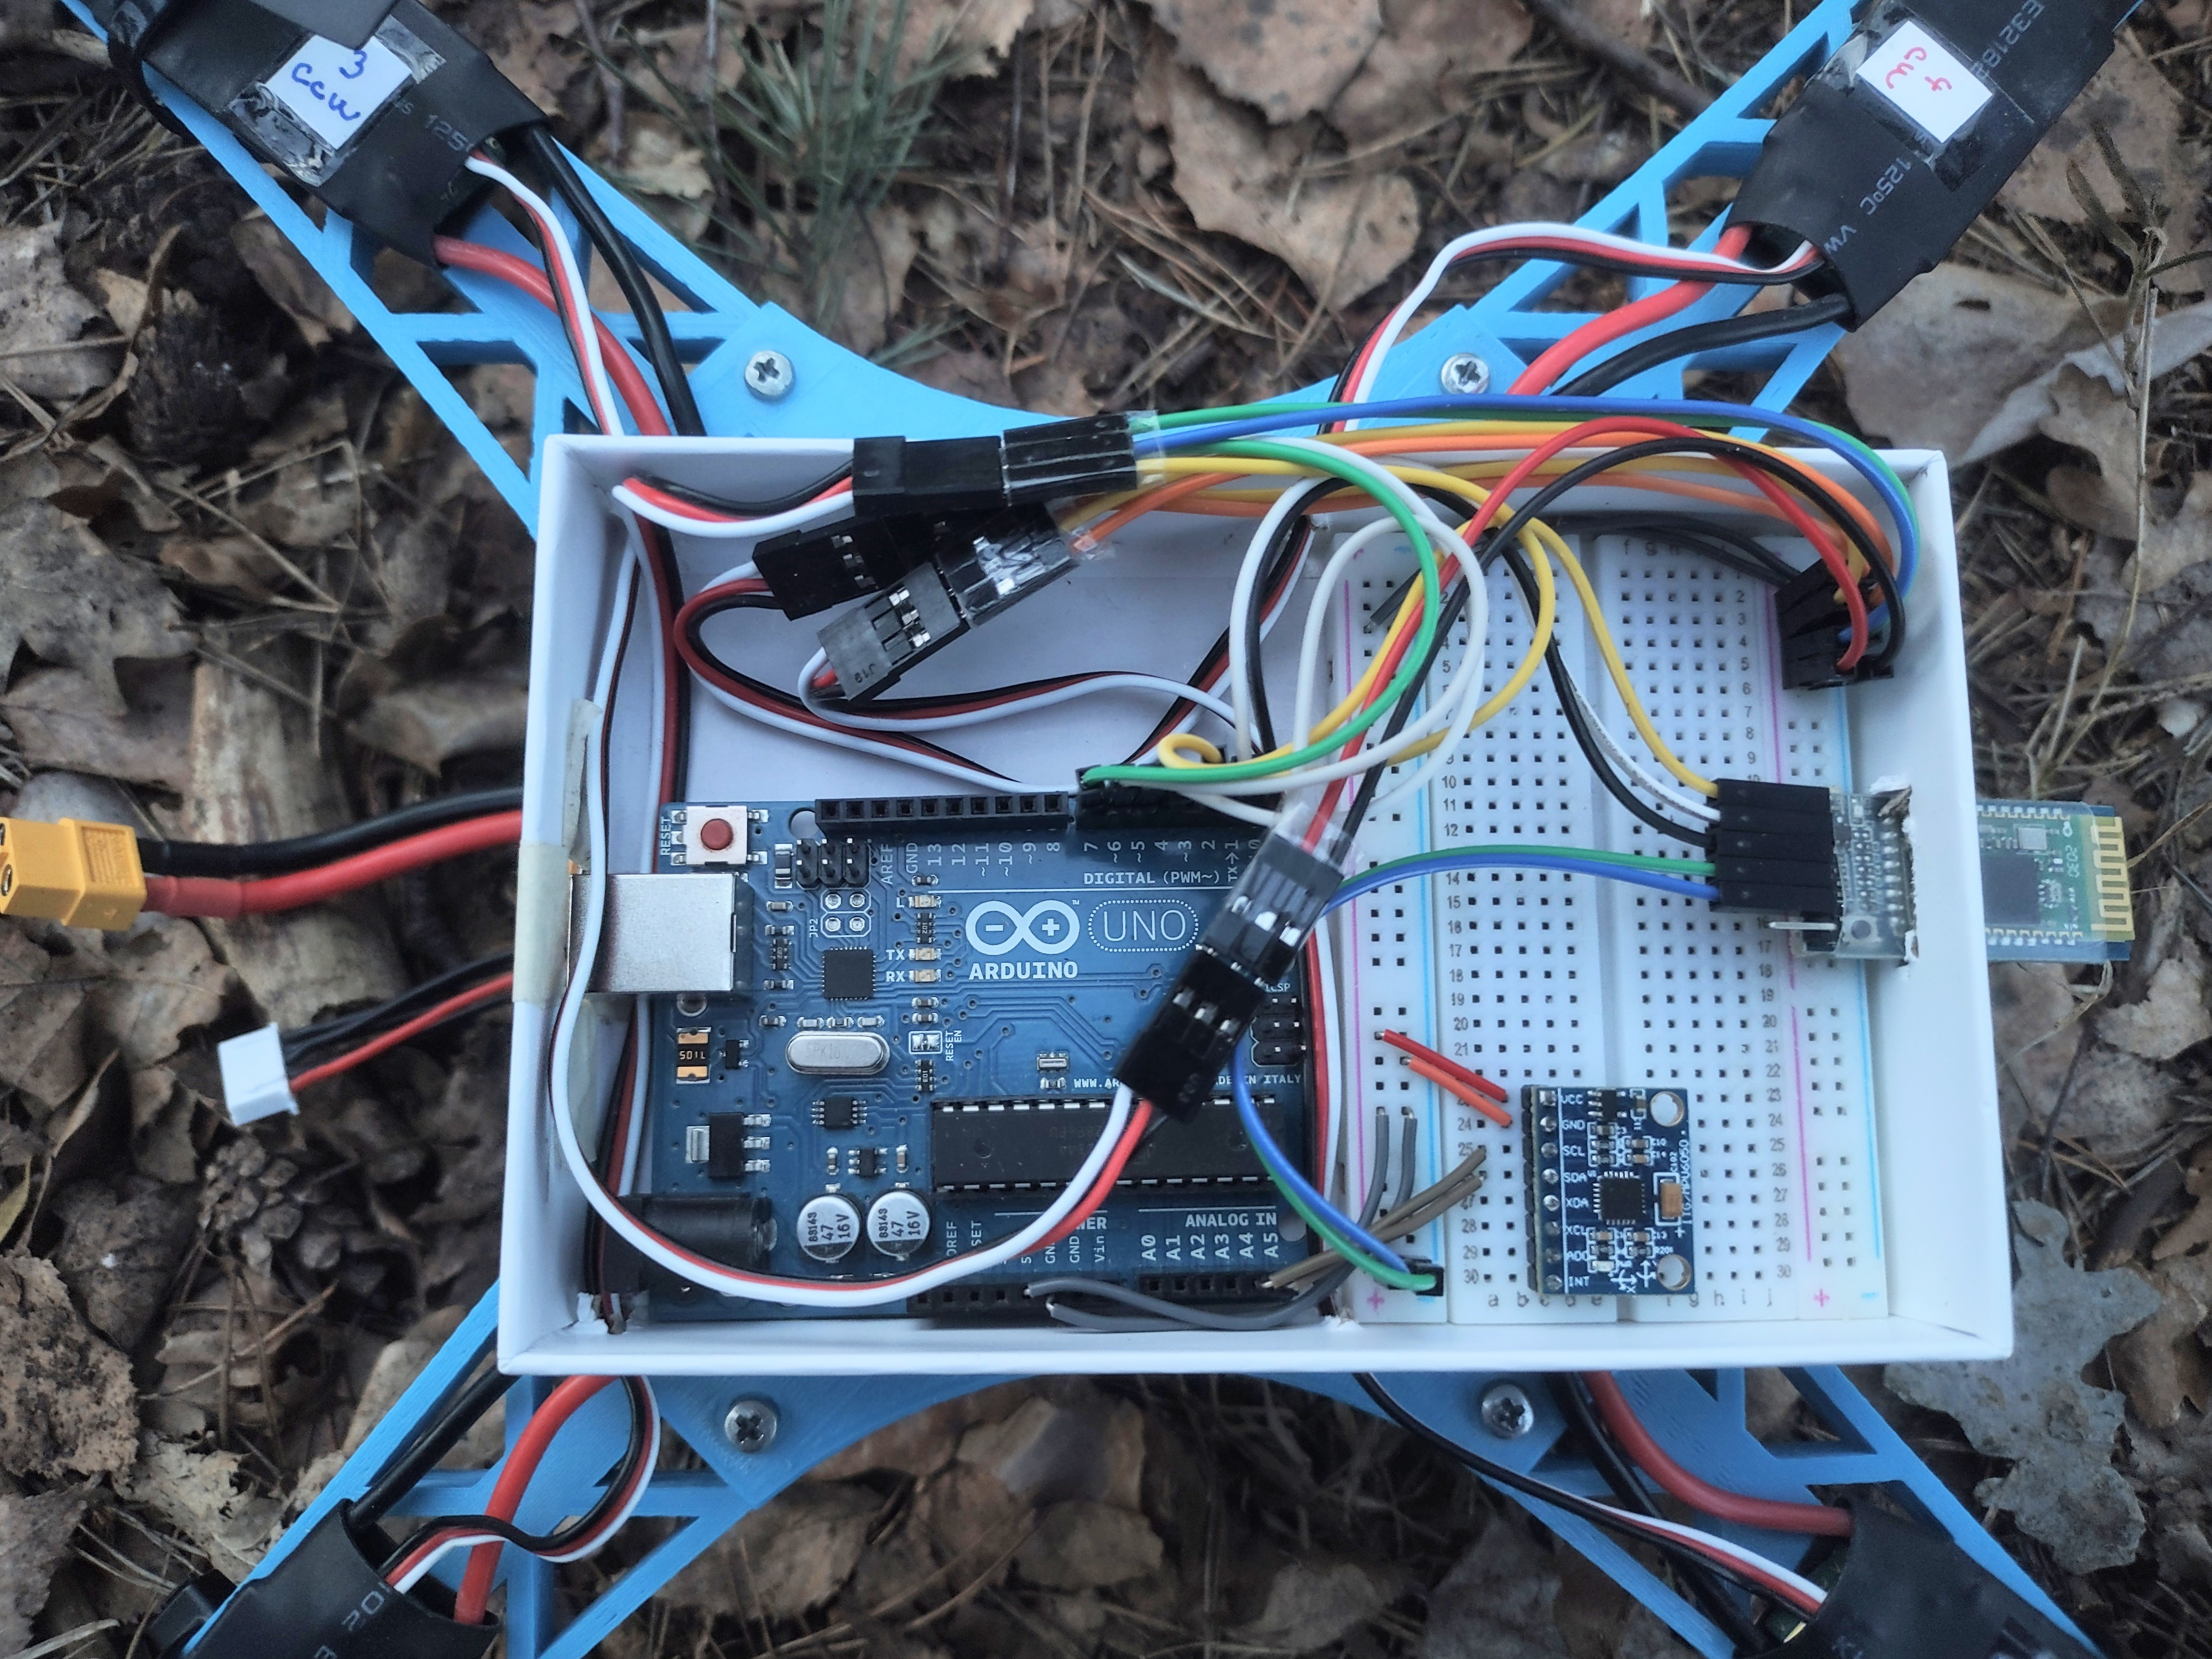
\includegraphics[width=0.75\linewidth]{ridici-jednotka.jpg}
	\caption{Řídicí jednotka ve své finální podobě v ochranném krytu}
	\label{fig:ridici-jednotka.jpg}
\end{figure}

\chapter[Program]{Program}
Program Arduina je navržen tak, aby umožňoval bezdrátové řízení kvadrokoptéry prostřednictvím mobilní aplikace Bluetooth Electronics. Program přijímá vysílané příkazy, analyzuje je a na jejich základě ovládá motory dronu. Každý ovládací prvek v aplikaci vysílá specifický signál s předponou, která umožňuje jeho správnou interpretaci.\\
\begin{figure}[H]
	\centering
	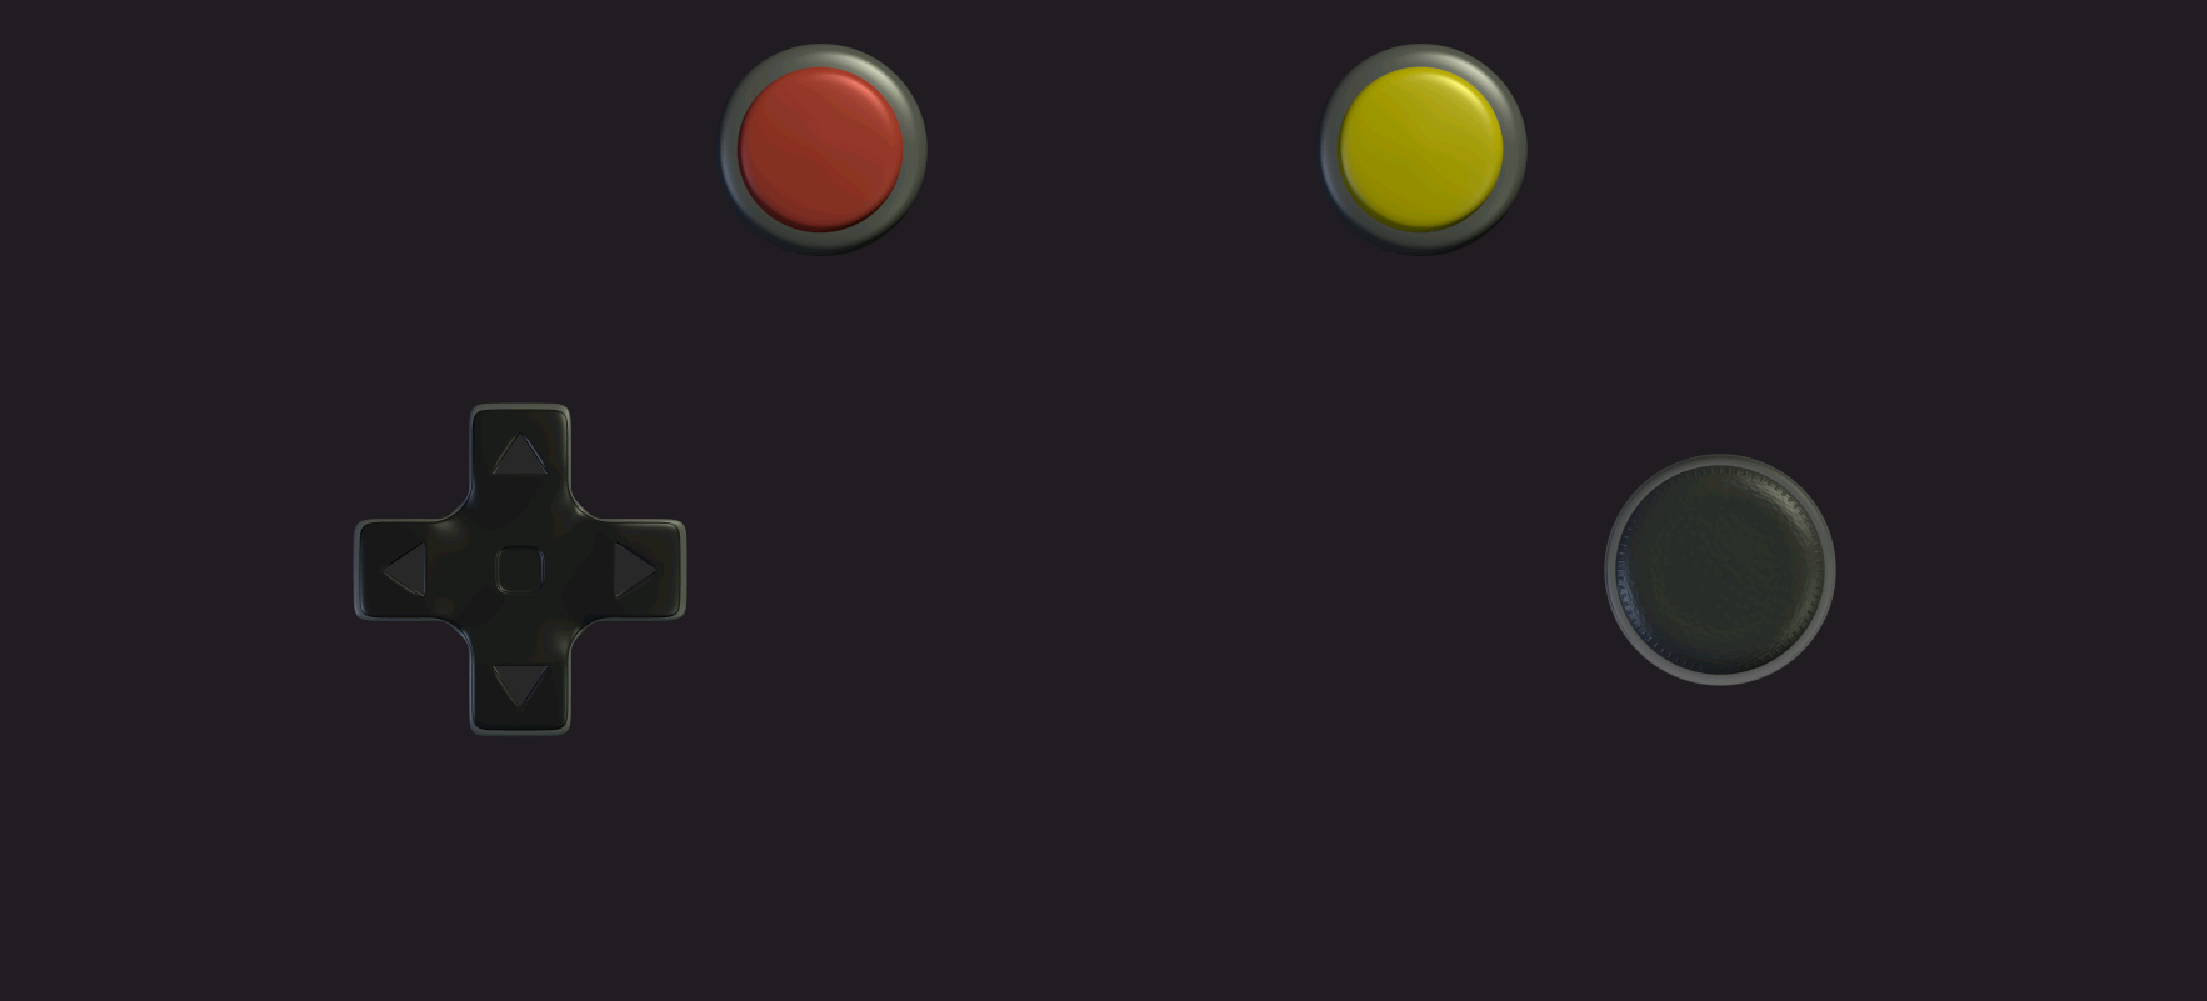
\includegraphics[width=0.75\linewidth]{aplikace.png}
	\caption{Snímek z ovládacího rozhraní v aplikaci Bluetooth Electronics}
	\label{fig:aplikace.png}
\end{figure}
Ovládání kvadrokoptéry je realizováno několika prvky. Směrová tlačítka umístěná na levé straně ovladače (ve tvaru „+“) vysílají příkazy s předponou \textit{p:} a číslem 1 až 4. Tlačítko šipky nahoru slouží ke zvýšení výkonu motorů, šipka dolů jej naopak snižuje. Směrová tlačítka vlevo a vpravo ovlivňují rotaci dronu kolem jeho vertikální osy.\\
K řízení směru letu slouží pravý joystick, jehož výchylka určuje náklon dronu. Ten odesílá příkazy s předponou \textit{m:} následovanou souřadnicemi X a Y, které odpovídají aktuální poloze joysticku na obrazovce mobilního zařízení. Na základě míry vychýlení joysticku se kvadrokoptéra nakloní v příslušném směru, čímž dochází ke změně trajektorie letu.\\
Důležitou součástí ovládacího systému jsou také bezpečnostní prvky. Červené tlačítko v horní části ovladače slouží jako nouzový vypínač a při jeho stisknutí dojde k okamžitému zastavení všech motorů. Žluté tlačítko zatím nemá přiřazenou žádnou funkci.\\
Pro vývoj a debugování provozu obsahuje program textový výstup, který umožňuje monitorování přijatých příkazů a jejich zpracování. Tyto informace lze zobrazit při připojení Arduina k počítači přes USB kabel. Program rovněž implementuje bezpečnostní mechanismus, který zajistí, že v případě ztráty spojení mezi mobilním zařízením a kvadrokoptérou dojde k okamžitému zastavení motorů.\\
Při nahrávání nového kódu do Arduina je nezbytné dočasně odpojit vodiče připojené k pinům 0 a 1, jelikož tyto piny jsou využívány v průběhu přenosu dat hardwarem Arduina. Po úspěšném nahrání je nutné vodiče znovu připojit na původní místo, aby mohla kvadrokoptéra správně komunikovat s mobilní aplikací. Další bezpečnostní opatření je součástí samotných motorů, které vyžadují, aby byl jejich výkon při startu nastaven na nulu. Teprve poté mohou být motory aktivovány.\\
Tento program tak umožňuje efektivní a bezpečné ovládání kvadrokoptéry, přičemž zohledňuje jak uživatelskou přívětivost, tak i bezpečnostní aspekty provozu.

\chapter[Schéma zapojení]{Schéma zapojení}
Propojení Arduina s Bluetooth modulem, akcelerometrem, gyroskopem, baterií, regulátory ESC a motory je znázorněné na obrázku schématu v programu Fritzing \cite{fritzing}. Celá pohonná soustava čerpá energii přímo z připojené baterie, zatímco samotné Arduino je napájeno přes ESC propojené s 5V pinem. Dva z bezkartáčových motorů mají odlišné zapojení vodičů, což způsobuje jejich rotaci opačným směrem.

\vspace{40pt}
\begin{figure}[H]
	\centering
	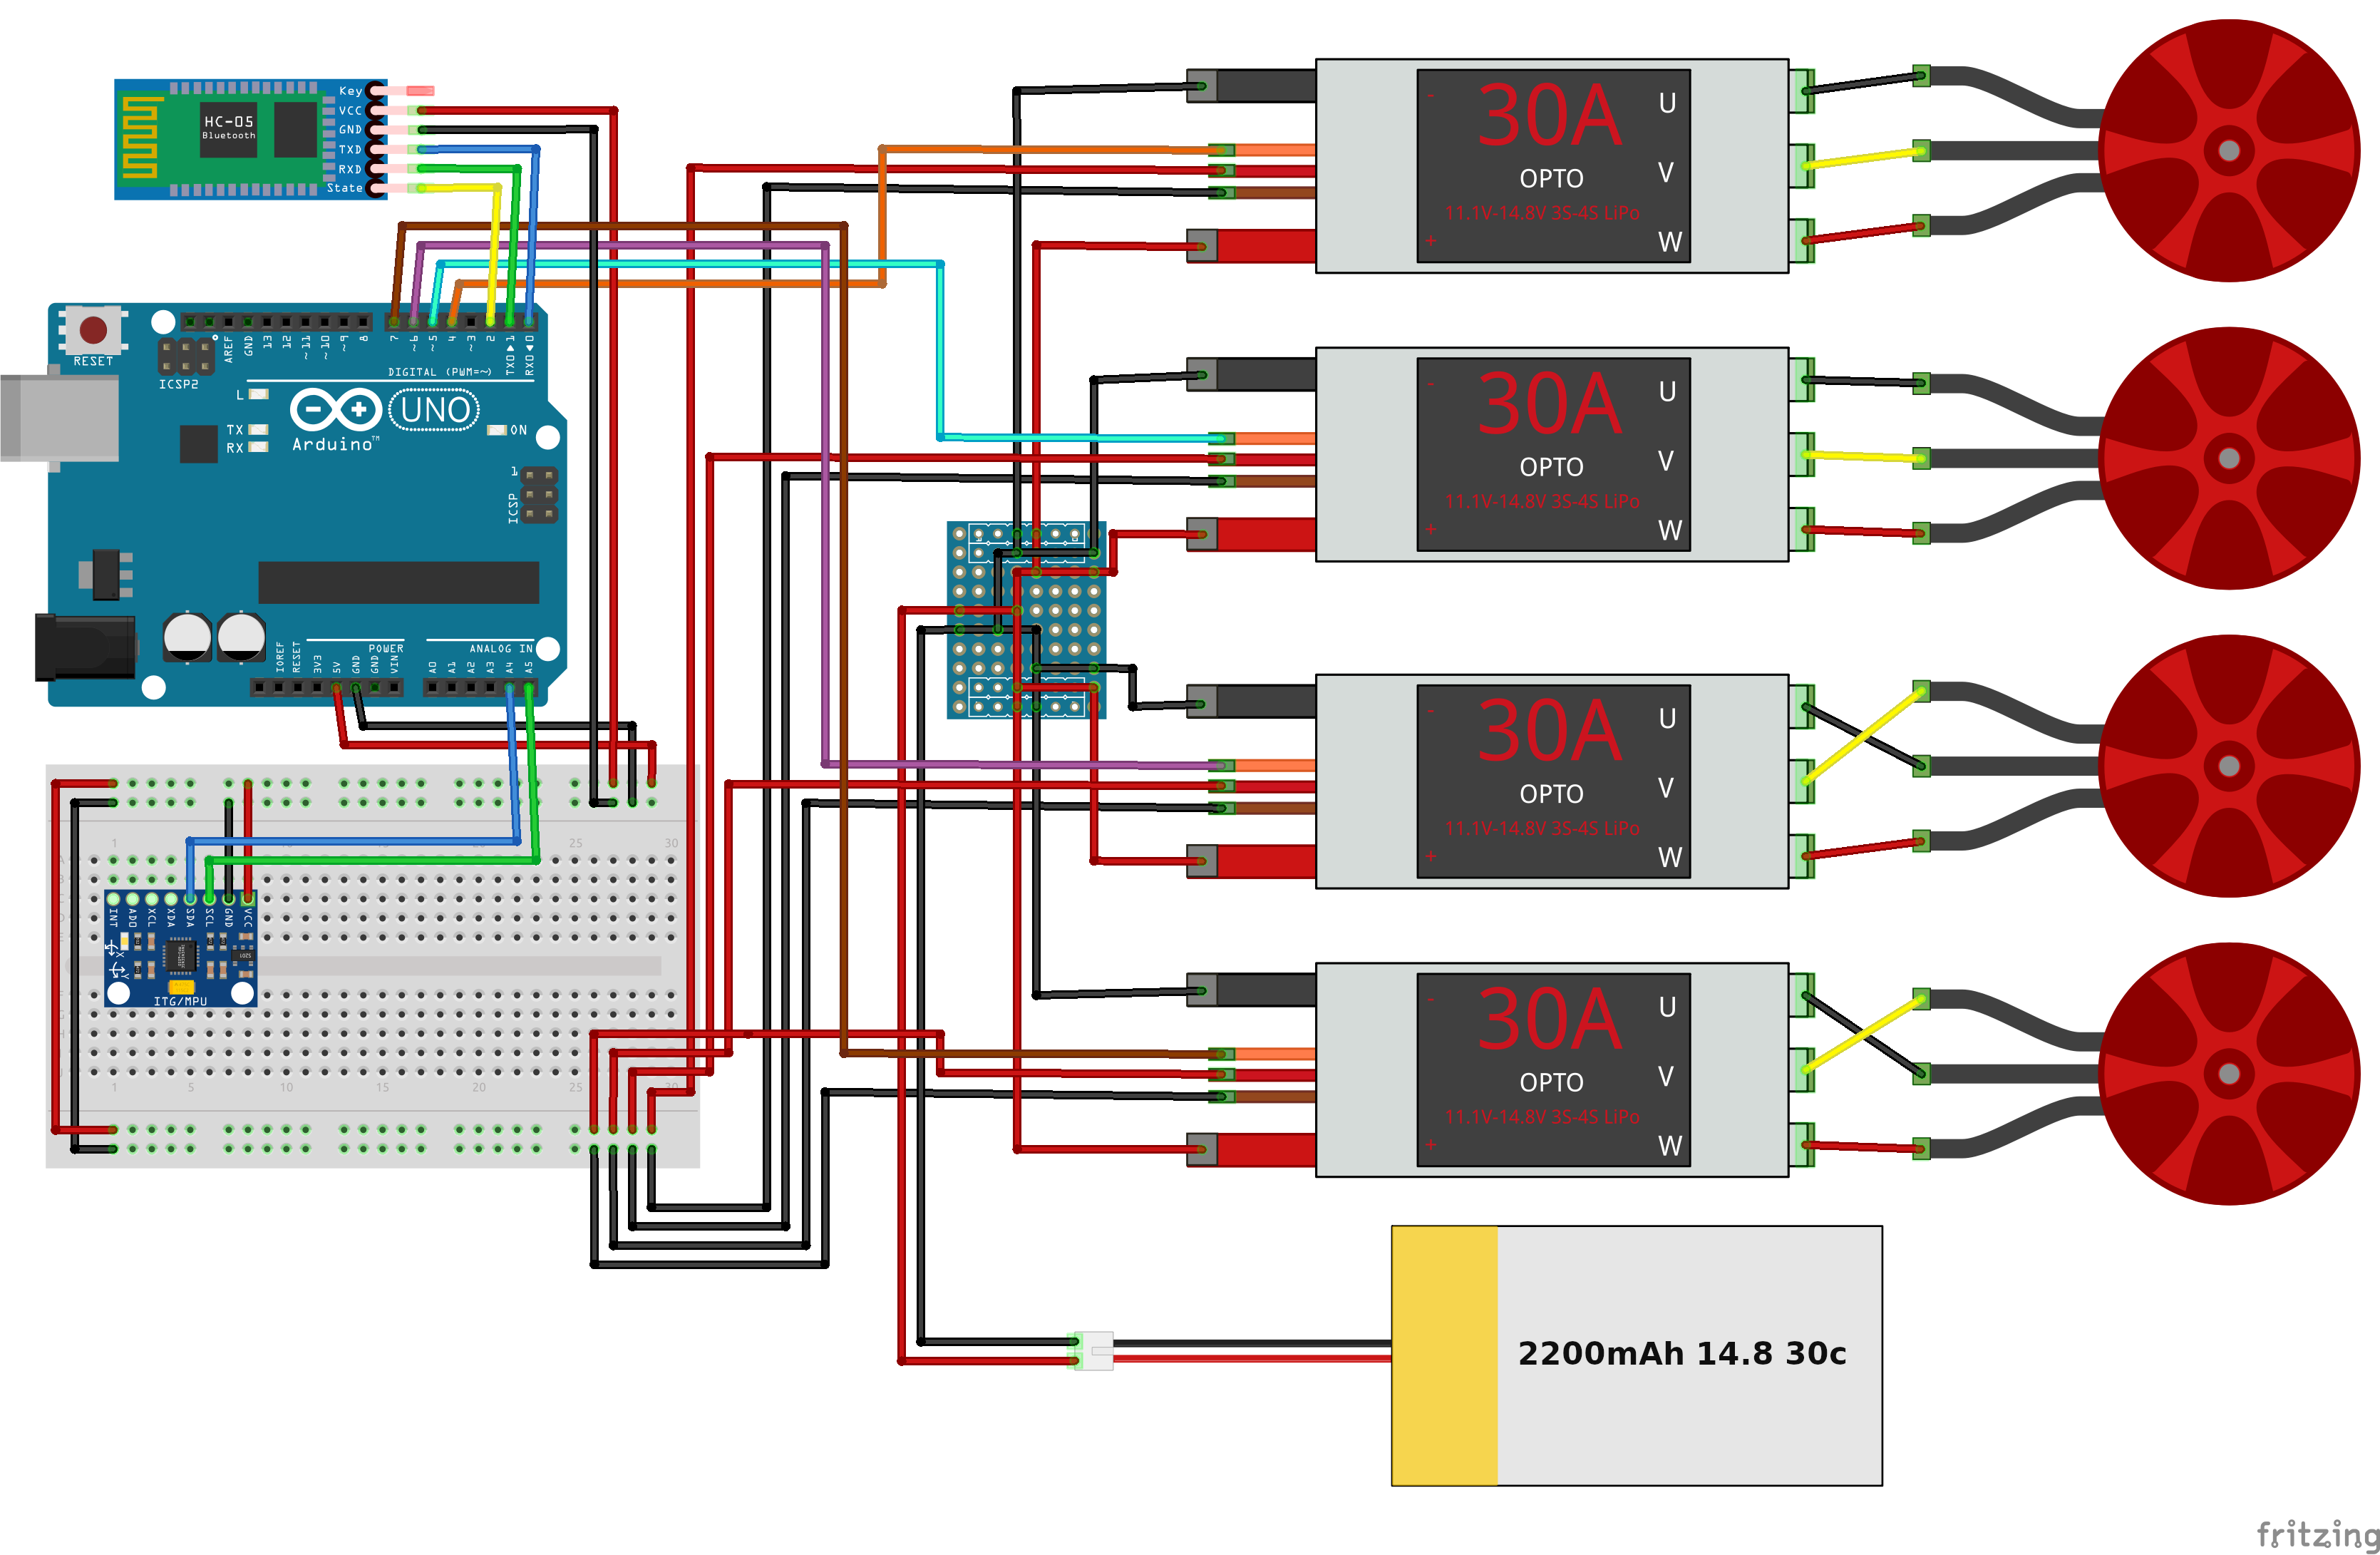
\includegraphics[width=\linewidth]{drone-scheme.png}
	\caption{Schéma propojení Arduina s moduly a pohonným systémem}
	\label{fig:drone-scheme.png}
\end{figure}

%%%%%%%%%%%%% ZÁVĚR
\chapter*{Závěr}
	
\lipsum[1]
	
\nocite{*}
\printbibliography					% Vytvoří seznam literatury
\addcontentsline{toc}{chapter}{Bibliografie}
\printglossary[title={Zkratky}]		% Vytvoří seznam zkratek
\listoffigures						% Vytvoří seznam obrázků

%%%%%%%%%%%%% PŘÍLOHY - APPENDIX 	
\begin{appendices}
\chapter[Fotografie zkonstruované kvadrokoptéry]{Fotografie zkonstruované kvadrokoptéry}	
\begin{figure}[H]
	\centering
	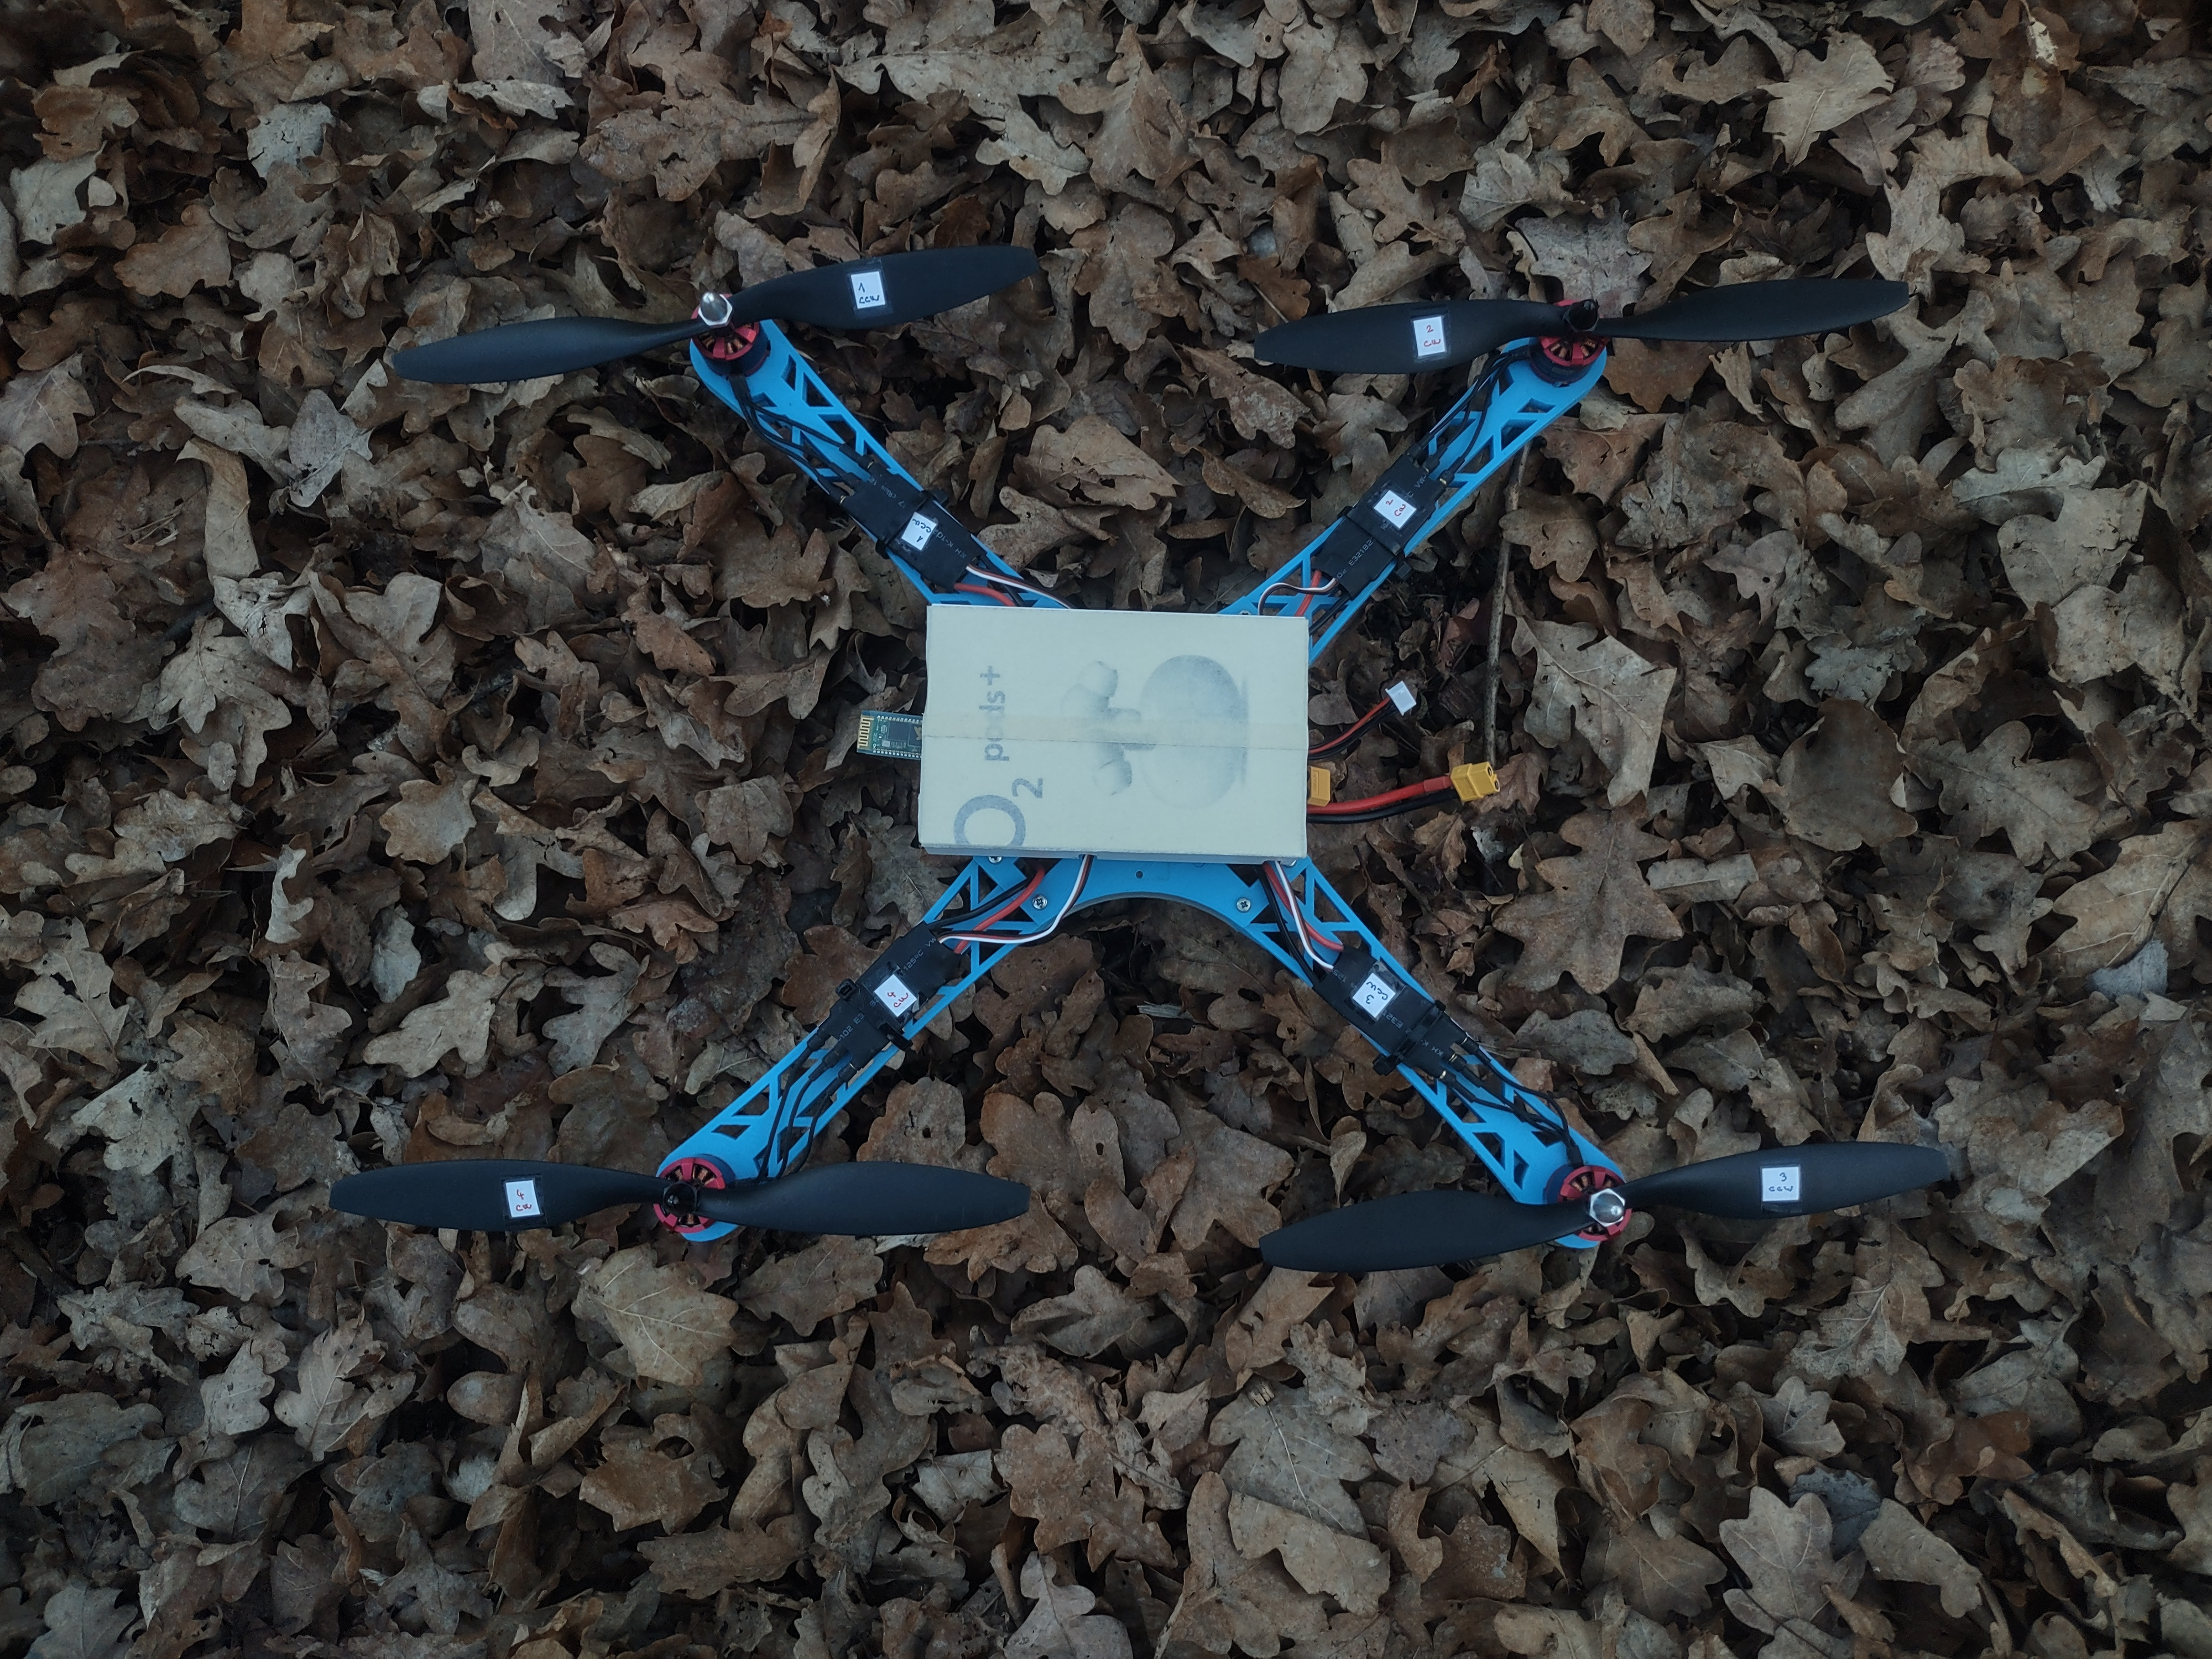
\includegraphics[width=\linewidth]{finalni-dron1.jpg}
\end{figure}
\begin{figure}[H]
	\centering
	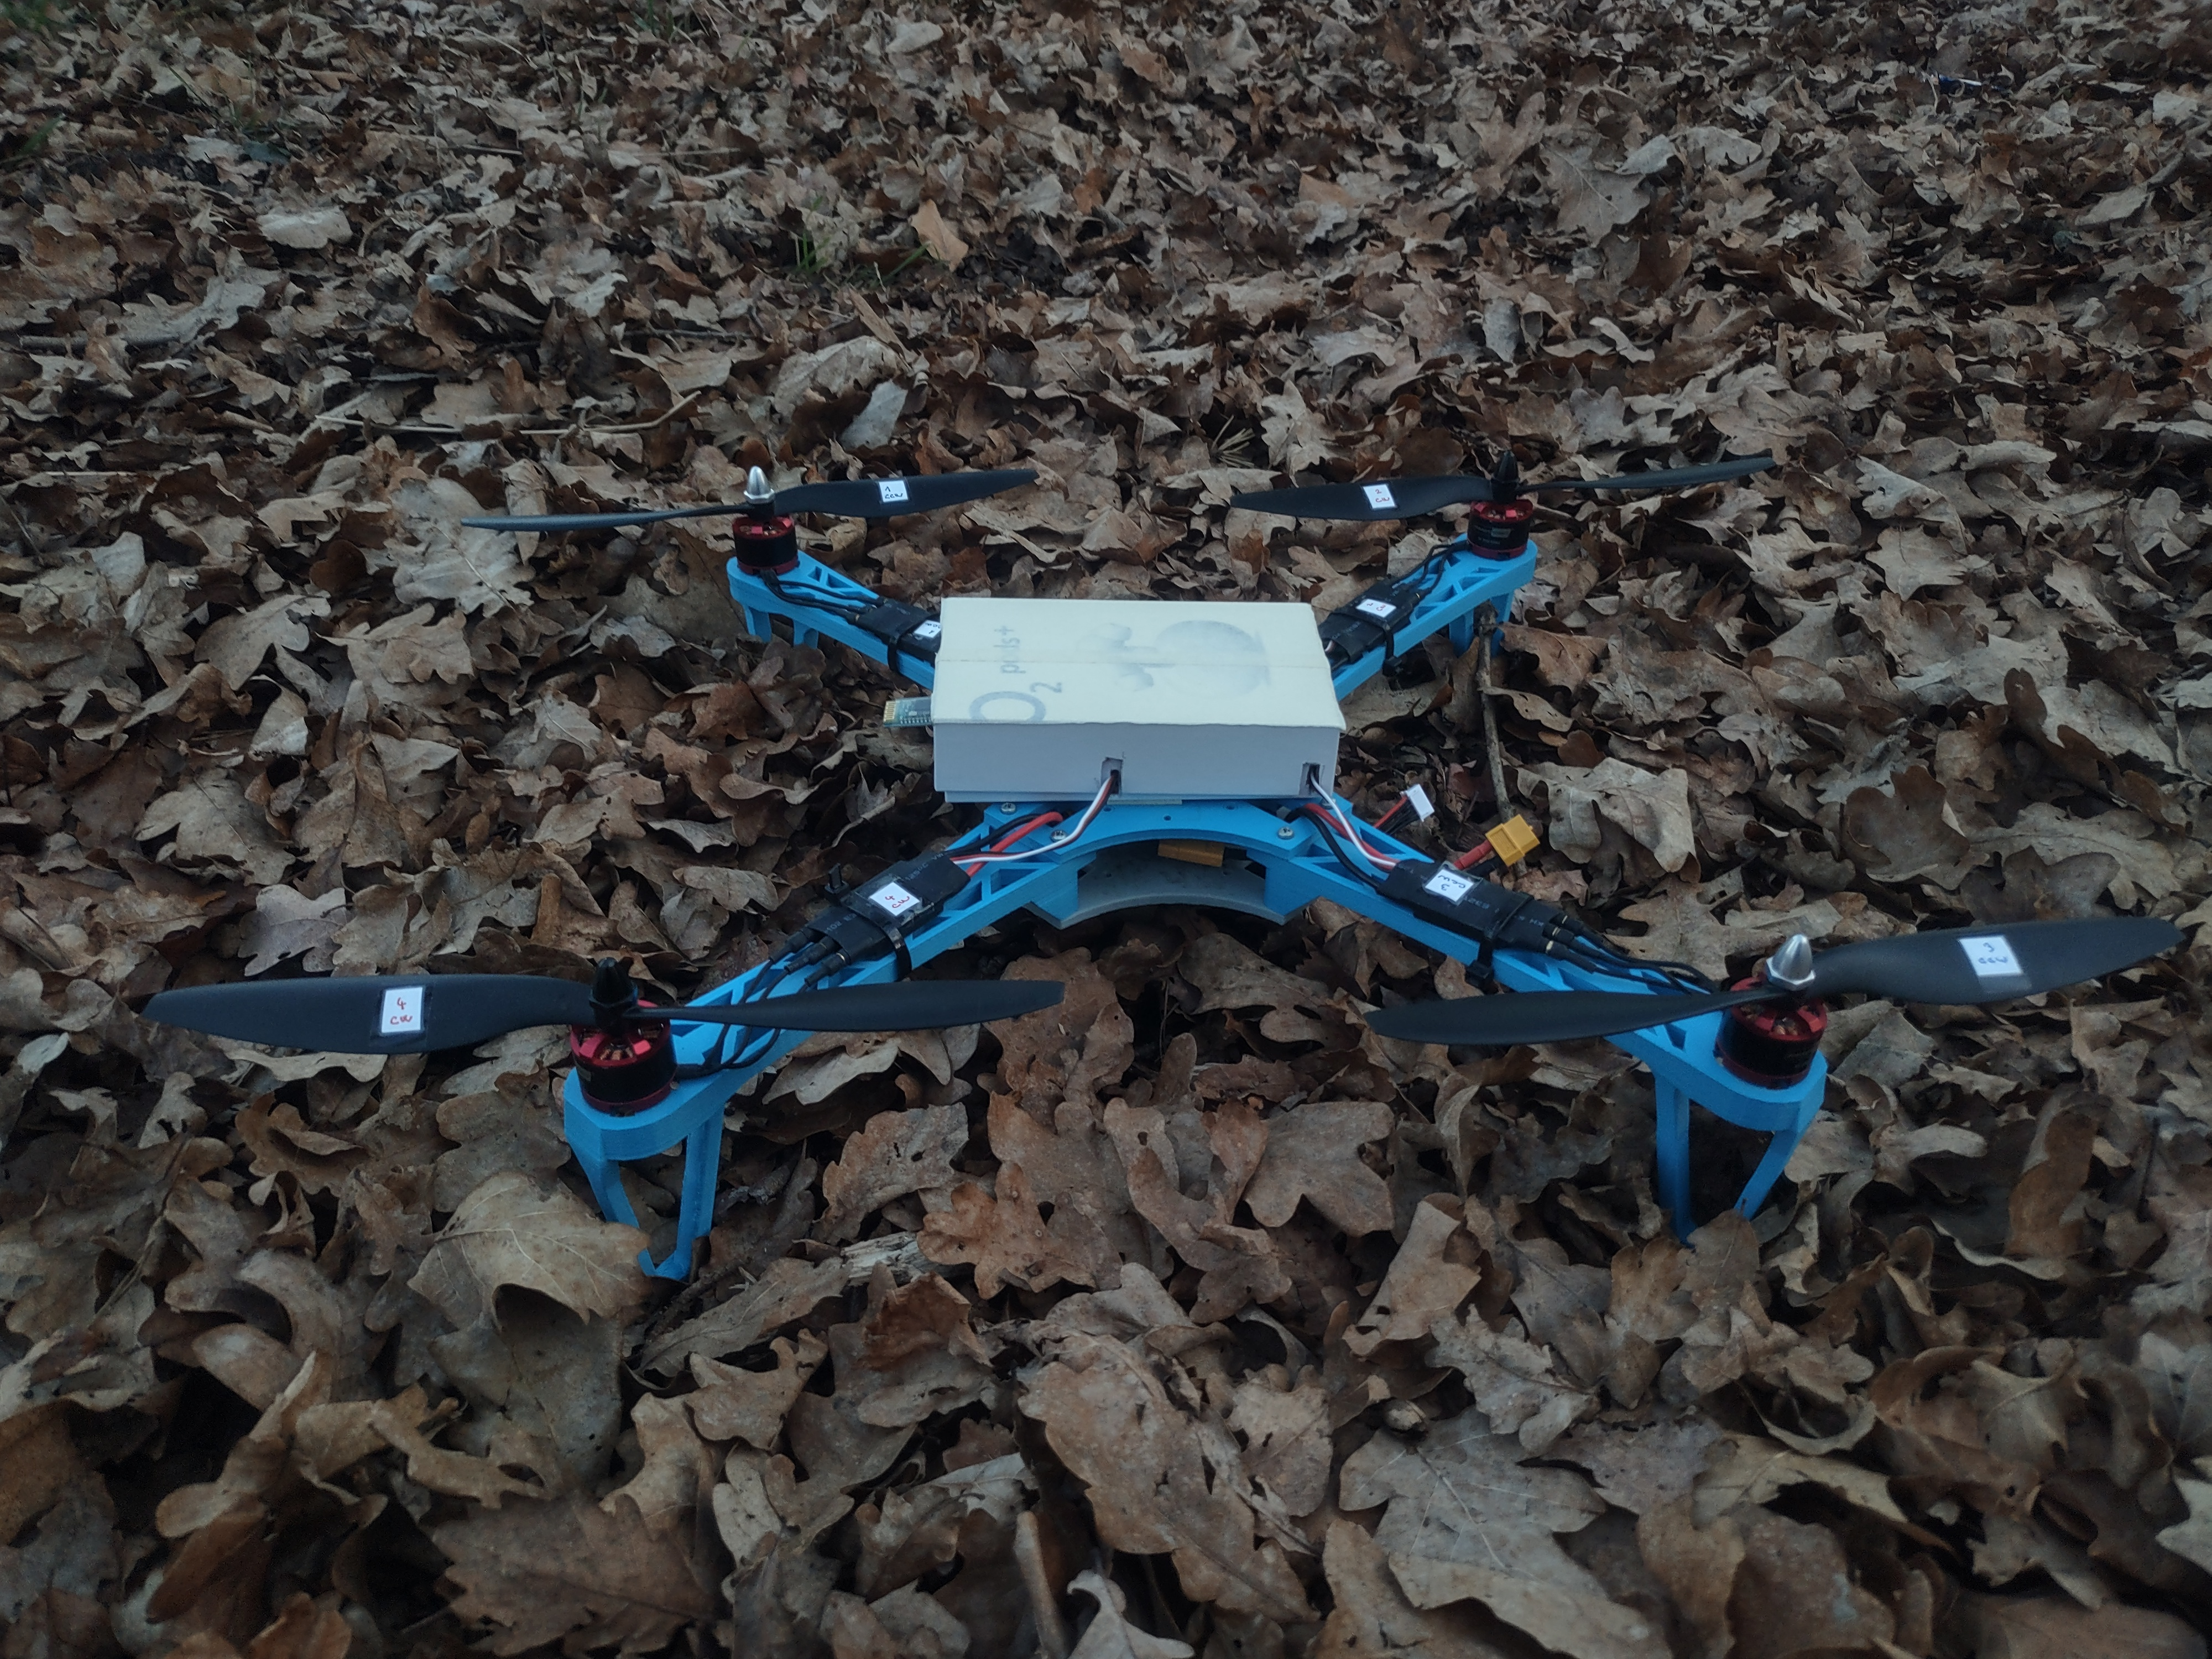
\includegraphics[width=\linewidth]{finalni-dron2.jpg}
\end{figure}
\chapter[Kód programu Arduina]{Kód programu Arduina}
\begin{lstlisting}[title={}, caption={}, label={}, basicstyle=\footnotesize\ttfamily, inputencoding=utf8]
#include <Servo.h> // Knihovna pro ovladani ESC pomoci PWM signalu

String data = ""; // Retezec pro ukladani prijatych dat pres Bluetooth
Servo ESC1;     // Vytvoreni objektu servo pro rizeni ESC motoru 1
Servo ESC2;
Servo ESC3;
Servo ESC4;
int power;      // Promenna pro ukladani vykonu motoru (0-100 %)
int escValue;   // Promenna pro prepocet vykonu na hodnotu pro ESC (0-180)
const int bluActive = 2; // Pin pro kontrolu stavu pripojeni Bluetooth modulu HC-05 (STATE pin)

void processCommand() {
// Zpracovani prikazu zacinajicich "p:"
if (data.startsWith("p:")) {
	String value = data.substring(2); // Extrahovani hodnoty po "p:"
	int number = value.toInt();       // Prevedeni na cele cislo

	Serial.print("Zpracovavam prikaz: p:");
	Serial.println(number);

	// Zvyseni vykonu motoru
	if (number == 1) {
	if (power <= 95) {
		power += 5;
		Serial.print("Vykon: ");
		Serial.println(power);
	} else {
		power = 100;
	}

	// Rotace doleva p:2 (zatim neimplementovano)
	} else if (number == 2) {
	Serial.println("Akce pro p:2");

	// Snizeni vykonu motoru
	} else if (number == 3) {
	if (power >= 5) {
		power -= 5;
		Serial.print("Vykon: ");
		Serial.println(power);
	} else {
		power = 0;
	}

	// Rotace doprava p:4 (zatim neimplementovano)
	} else if (number == 4) {
	Serial.println("Akce pro p:4");

	} else {
	Serial.println("Neznamy prikaz po p:");
	}
}

// Zpracovani prikazu zacinajicich "b:"
else if (data.startsWith("b:")) {
	String value = data.substring(2); // Extrahovani hodnoty po "b:"
	int number = value.toInt();       // Prevedeni na cele cislo

	Serial.print("Zpracovavam prikaz: b:");
	Serial.println(number);

	// Zastaveni vsech motoru
	if (number == 0) {
	Serial.println("Tlacitko b0 stisknuto");
	power = 0;
	// Neimplementovana funkcionalita druheho tlacitka
	} else if (number == 1) {
	Serial.println("Tlacitko b1 stisknuto");
	} else {
	Serial.println("Neznamy prikaz b:");
	}
}

// Zpracovani prikazu zacinajicich "m:"
// Naklon dopredu, do zadu a dostran (zatim neimplementovano)
else if (data.startsWith("m:")) {
	int xIndex = data.indexOf('X'); // Najiti pozice 'X'
	int yIndex = data.indexOf('Y'); // Najiti pozice 'Y'

	if (xIndex != -1 && yIndex != -1) { // Overeni, ze obe hodnoty existuji
	String xValue = data.substring(xIndex + 1, yIndex); // Extrahovani hodnoty X
	String yValue = data.substring(yIndex + 1);         // Extrahovani hodnoty Y

	int x = xValue.toInt(); // Prevedeni hodnoty X na cele cislo
	int y = yValue.toInt(); // Prevedeni hodnoty Y na cele cislo

	Serial.print("X: ");
	Serial.println(x);
	Serial.print("Y: ");
	Serial.println(y);

	Serial.println("Zpracovavam prikaz m:...");
	} else {
	Serial.println("Neplatny format prikazu m:");
	}
}

// Ignorovani zprav, ktere nezacinaji "p:", "b:", nebo "m:"
else {
	Serial.println("Zprava ignorovana (neznamy format)");
}

// Vymazani datoveho retezce pro dalsi zpravy
data = "";
}

void setup() {
Serial.begin(9600); // Spusteni seriove komunikace
Serial.println("Pripraveno na prijem dat pres Bluetooth...");

// Pripojeni ESC motoru na piny 4-7
ESC1.attach(4, 1000, 2000); // (pin, min sirka pulzu, max sirka pulzu v mikrosekundach)
ESC2.attach(5, 1000, 2000);
ESC3.attach(6, 1000, 2000);
ESC4.attach(7, 1000, 2000);

power = 0; // Vychozi vykon motoru
pinMode(bluActive, INPUT); // Nastaveni pinu pro cteni stavu Bluetooth pripojeni
}

void loop() {
// Kontrola, zda je k dispozici data ze seriove komunikace
if (Serial.available() > 0) {
	char incomingChar = Serial.read(); // Precteni znaku z Bluetooth

	if (incomingChar == '\n') { // Kontrola konce zpravy (novy radek)
	Serial.print("Prijata zprava: ");
	Serial.println(data); // Vypsani prijate zpravy
	processCommand(); // Zpracovani prijateho prikazu
	} else {
	data += incomingChar; // Pridani znaku do retezce zpravy
	}
}

// Kontrola stavu Bluetooth pripojeni
int connectionStatus = digitalRead(bluActive); // Cteni pinu STATE z HC-05
if (connectionStatus == LOW) { // Pokud je stav LOW, Bluetooth je odpojeno
	power = 0; // Reset vykonu motoru na vychozi hodnotu
	Serial.println("Bluetooth odpojeno!");
}

// Prevod vykonu (0-100) na hodnotu (0-180) pro ESC motory
escValue = map(power, 0, 100, 0, 180); 
ESC1.write(escValue); // Nastaveni vykonu pro motor 1
ESC2.write(escValue);
ESC3.write(escValue);
ESC4.write(escValue);
}	
\end{lstlisting}  
\end{appendices}
%%%%%%%%%%%%%%%
\end{document}
%%%%%%%%%%%%%%%%%%%% KONEC %%%%%%%%%%%%%%%%%%%%%%%%%